% TODO: Bei den SET examples koennte man parallel das
%       Ergenis zeigen:
%       set A := { 1..4}     |  { 1, 2, 3, 4 }
%
%       min/max expr beispiel
%
%\section{Introduction}


%% Consider the following linear program:
%% $$
%% \begin{array}{rll}
%% \min& 2 x + 3 y\\
%% \mbox{subject to}& x + y& \leq 6\\
%% &x,y&\ge 0\\
%% \end{array}
%% $$
%% The standard format used to feed such a problem into a solver
%% is called \mps.
%% \ibm invented it for the Mathematical
%% Programming System/360 \cite{Kallrath2004b,Spielberg2004} in the sixties.
%% Nearly all available \lp and \mip solvers can read this format.
%% While \mps is a nice format to punch into a punch card and at least a
%% reasonable format to read for a computer, it is quite unreadable
%% for humans. For instance, the \mps file of the above linear program
%% looks as follows:

%% \medskip
%% \lstset{language=mps,%
%% basicstyle=\sffamily\footnotesize,%
%% numberstyle=\sffamily\tiny\color{siennabrown},stepnumber=1}
%% \begin{lstlisting}[frame=]{}
%%     NAME        ex1.mps
%%     ROWS
%%      N  OBJECTIV
%%      L  c1
%%     COLUMNS
%%         x         OBJECTIV             2
%%         x         c1                   1
%%         y         OBJECTIV             3
%%         y         c1                   1
%%     RHS
%%         RHS       c1                   6
%%     BOUNDS
%%      LO BND       x                    0
%%      LO BND       y                    0
%%     ENDATA
%% \end{lstlisting}

%% \bigskip
%% \noindent Another possibility is the \lpf format \cite{CPlex80}, which is more
%% readable\footnote{
%% The \lpf format has also some idiosyncratic restrictions. For example
%% variables should not be named \code{e12} or the like. And it is not
%% possible to specify ranged constraints.}
%% but is only supported by a few solvers.
%% {
%% \small
%% \begin{verbatim}
%%    Minimize
%%     cost:  +2 x +3 y
%%    Subject to
%%     c1:  +1 x +1 y <= 6
%%    End
%% \end{verbatim}
%% }
%% \noindent But since each coefficient of the matrix $A$ must be stated
%% explicitly it is also not a desirable choice to develop a mathematical
%% model.

%% \medskip
%% \noindent Now, with \zimpl it is possible to write this:
%% {\small
%% \begin{verbatim}
%%    var x;
%%    var y;
%%    minimize cost: 2 * x + 3 * y;
%%    subto c1: x + y <= 6;
%% \end{verbatim}
%% }
%% \noindent and have it automatically translated into \mps or \lpf format.
%% While this looks not much different from what is in the \lpf format,
%% the difference can be seen, if we use indexed variables.
%% Here is an example. This is the \lp:
%% $$
%% \begin{array}{rl}
%% \min& 2 x_1 + 3 x_2 + 1.5 x_3\\
%% \mbox{subject to}&\sum^3_{i=1} x_i \leq 6\\
%% &x_i\ge 0\\
%% \end{array}
%% $$
%% And this is how to tell it to \zimpl:

%% \medskip
%% \lstset{language=zimpl,%
%% basicstyle=\sffamily\footnotesize,%
%% numberstyle=\sffamily\tiny\color{siennabrown},stepnumber=1}
%% \begin{lstlisting}[frame=]{}
%%    set I      := { 1 to 3 };
%%    param c[I] := <1> 2, <2> 3, <3> 1.5;
%%    var   x[I] >= 0;
%%    minimize cost: sum <i> in I : c[i] * x[i];
%%    subto    cons: sum <i> in I : x[i] <= 6;
%% \end{lstlisting}



\clearpage

\section{简介}
% \section{Introduction}

考虑一个$s-t$最短路问题的线性规划形式,针对有向图$(V, A)$,边的成本系数
记为 $c_{ij}$,对于集合$A$中的所有边 $(i, j) \in A$,建模如下:
% Consider the \lpf formulation of the shortest $s,t$-path problem,
% applied to some directed graph $(V,A)$ with cost coefficient $c_{ij}$
% for all $(i,j) \in A$:

\begin{equation}
  \begin{array}{rll}
    \min& \displaystyle\sum_{(i,j) \in A} c_{ij} x_{ij}\\
    & \displaystyle\sum_{(iv)\in \delta^-(v)} x_{iv} = \sum_{(vi)\in
      \delta^+(v)} x_{vi}
       \mbox{\quad for all }v \in V\setminus\{s,t\} \\
       &  \\
    & x_{ij} \in \{0,1\}, \mbox{for all {i,j} in A}\\
  \end{array}\label{eq:shortestpath}
\end{equation}
%
其中,对于任意$v \in V$,定义$\delta^+(v) := {(v, i) \in A}$和
$\delta^-(v) := {(i, v) \in A}$。对于一个特定的图,模型可以具象表述为:
% where $\delta^+(v):=\{(v,i) \in A\}$, $\delta^-(v):=\{(i,v) \in A\}$
% for $v\in V$. For a given graph  the instantiation is

\begin{minipage}[c]{0.3\linewidth}
  \begin{center}
    \label{stexample}
    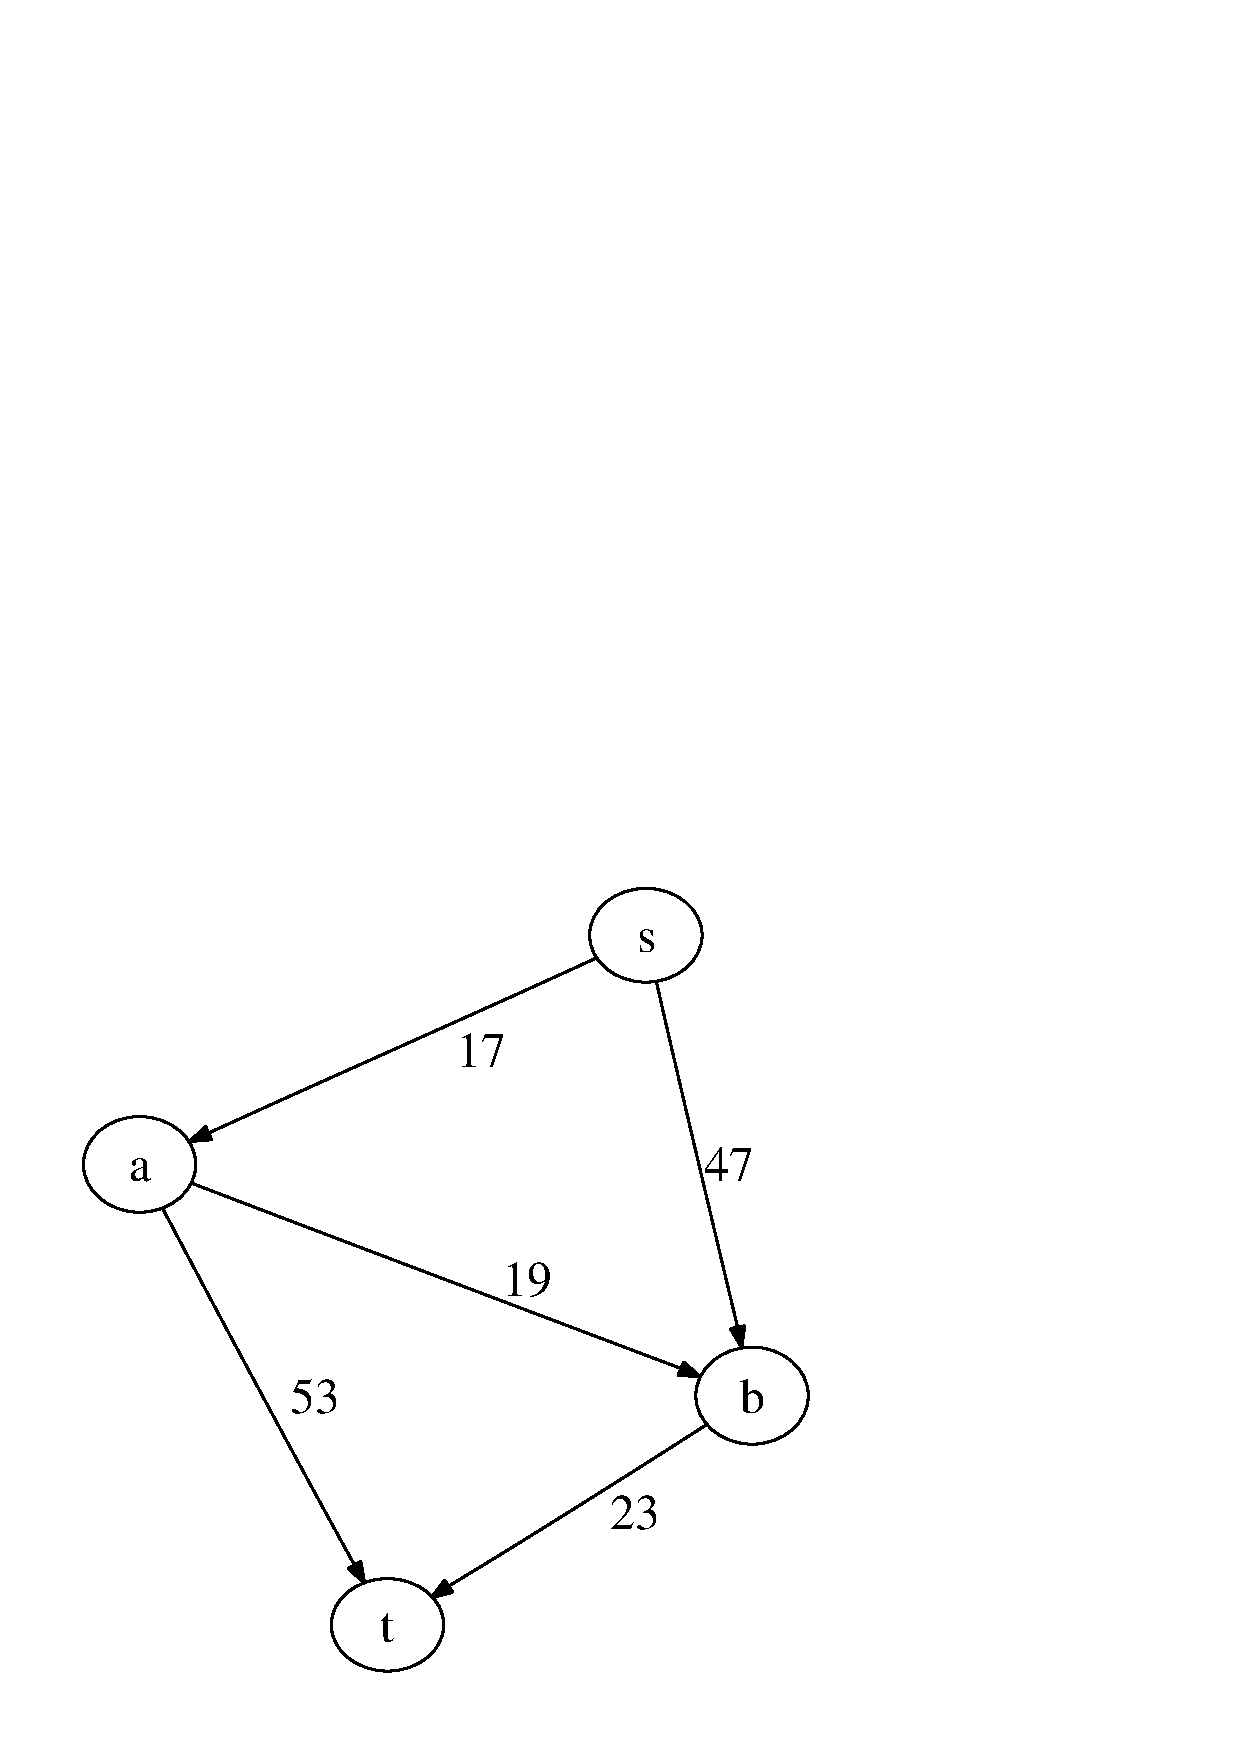
\includegraphics[height=4cm]{stexample}
  \end{center}
\end{minipage}
%
\begin{minipage}[c]{0.5\linewidth}
  $$
   \begin{array}{rll}
    \min& 17 x_{sa} + 47 x_{sb} + 19 x_{ab} + 53 x_{at} + 23 x_{bt}     \\
    \mbox{subject to}& x_{sa} = x_{ab} + x_{at} \\
    & x_{sb} + x_{ab} = x_{bt} \\
    &x_{ij} \in \{0,1\}, \mbox{for all {i,j}}\\
  \end{array}
  $$
\end{minipage}

现将此类问题输入求解器所使用的标准格式称为\mps,这一格式系\ibm 为20世纪60
年代的数学规划系统 System/360 设计的~\cite{Kallrath2004b,Spielberg2004}。
尽管几乎所有现存的线性规划 (\lp) 和混合整数规划 (\mip) 求解器都能读取这种
格式,虽然\mps 格式非常适合通过穿孔纸带输入,且对计算机来说也至少是可读的
,但对人类而言,却几乎不可理解。例如上述线性规划问题的\mps 文件内容如下:
% The standard format used to feed such a problem into a solver is
% called \mps which was invented by \ibm for the Mathematical
% Programming System/360 in the
% sixties~\cite{Kallrath2004b,Spielberg2004}.  Nearly all available \lp
% and \mip solvers can read this format.  While \mps is a nice format to
% punch into a punch card and at least a reasonable format to read for a
% computer, it is quite unreadable for humans. For instance, the \mps
% file of the above linear program looks as follows:

\lstset{language=mps,%
basicstyle=\sffamily\footnotesize,%
numberstyle=\sffamily\tiny\color{siennabrown},stepnumber=1}
\begin{lstlisting}[frame=]{}
NAME          shortestpath.lp
ROWS
 N  Obj
 E  c0
 E  c1
 E  c2
COLUMNS
    INTSTART  'MARKER'       'INTORG'
    x0        Obj        17  c0            1
    x0        c2          1
    x1        Obj        47  c1            1
    x1        c2          1
    x2        c1          1  c0           -1
    x2        Obj        19
    x3        Obj        53  c0           -1
    x4        c1         -1  Obj          23
RHS
    RHS       c2          1
BOUNDS
 UP Bound     x0          1
 UP Bound     x1          1
 UP Bound     x2          1
 UP Bound     x3          1
 UP Bound     x4          1
ENDATA
\end{lstlisting}

\bigskip
\noindent 而另一个可能的格式是\lpf 格式\cite{CPlex80}相比之下具有更高的可
读性\footnote{\lpf 格式也具有一些乖张的限制。比如变量不能被命名为
  \code{e12}或者类似的名称,而且也不能指定范围约束。},很接近具象化的表述
  ,但是只被极少数的求解器所支持。
% \noindent Another possibility is the \lpf format \cite{CPlex80} which
% is more readable\footnote{ The \lpf format has also some idiosyncratic
%   restrictions. For example variables should not be named \code{e12}
%   or the like. and it is not possible to specify ranged
%   constraints.}, quite similar to the instantiation,
% but only supported by a few solvers:
{ \small
\begin{verbatim}
Minimize
 Obj: +17 x0 +47 x1 +19 x2 +53 x3 +23 x4
Subject to
 c0: -1 x3 -1 x2 +1 x0 = +0
 c1: -1 x4 +1 x2 +1 x1 = +0
 c2: +1 x1 +1 x0 = +1
Bounds
 0 <= x0 <= 1
 0 <= x1 <= 1
 0 <= x2 <= 1
 0 <= x3 <= 1
 0 <= x4 <= 1
Generals
 x0 x1 x2 x3 x4
End
\end{verbatim}
}
\noindent 而鉴于其中又必须精确指定矩阵~$A$的每个参数,这仍算不上是一种数学
建模语言的理想选择。
% \noindent Since each coefficient of the matrix~$A$ must be stated
% explicitly it is also not a desirable choice for the development of a
% mathematical model.

\subsubsection{抽象公式表述}
% \subsubsection{Abstract formulation}

而现在,这一模型在\zimpl 中可以写作:
% Now, with \zimpl it is possible to write

{\small
\begin{verbatim}
set V      :={"a","b","s","t"};
set A      :={<"s","a">, <"s","b">, <"a","b">, <"a","t">, <"b","t">};
param c[A] := <"s","a"> 17, <"s","b"> 47, <"a","b"> 19, <"a","t"> 53,
              <"b","t"> 23;
defset dminus(v) := {<i,v> in A};
defset dplus(v)  := {<v,j> in A};
var x[A] binary;
minimize cost: sum<i,j> in A: c[i,j] * x[i,j];
subto fc:
      forall <v> in V - {"s","t"}:
        sum<i,v> in dminus(v): x[i,v] == sum<v,i> in dplus(v): x[v,i];
subto uf:
      sum<s,i> in dplus("s"): x[s,i] == 1;
\end{verbatim}
}

\noindent ——请将这段代码与~(\ref{eq:shortestpath}) 相比较。将这段代码输
入\zimpl 即可自动生成\mps 或\lpf 文件。
% \noindent -- compare this with~(\ref{eq:shortestpath}). Feeding the
% script into \zimpl will automatically generate \mps or \lpf files.


\medskip

像\zimpl 这样的建模语言的价值在于它们具备直接处理数学模型本身的能力,而不
是仅仅对系数进行处理。除此之外,模型的具象 (可以理解为是生成的\lpf 文件或
\mps 文件) 通常会通过外部数据生成。从某种意义上来讲,“具象化”正是将模型
应用于外部数据的结果。在我们上面的算例中,所谓外部数据就是带有成本系数和指
定的$s$和$t$的图,而模型则是$st$最短路优化问题的数学公式。当然,\zimpl 也
支持通过文件来初始化模型。例如,上述这个\zimpl 脚本的第一行也可以写作:%
% The value of modeling languages like \zimpl lies in their ability to
% work directly on the mathematical model in lieu of dealing merely with
% coefficients. Furthermore, more often than not instantiations (read
% \lpf or \mps-files) of models are generated from some external
% data. In some sense, these are the result of the model applied to this
% external data. In our example above, the external data is the graph
% together with the cost coefficients and the specification of $s$ and
% $t$, and the model is the formulation of the shortest $st$-path
% problem. Of course, \zimpl supports the initialization of models
% from files. For instance, the first lines from the \zimpl script above
% can be replaced by {\small
{\small
\begin{verbatim}
set       V:= {read "nodes.txt" as "<1s>"};
set       A:= {read "arcs.txt"  as "<1s,2s>"};
param c[A] := read "arcs.txt"  as "<1s,2s>3n";
\end{verbatim}
} 而\zimpl 也可以根据“nodes.txt”和“arcs.txt”两个文件中的定义生成任何一
个最短路问题的实例。这些文件中具体的格式规定将在\ref{initfromfile}节中叙述。
% } and the \zimpl script is ready produce instances of any shortest
% path problem defined by the files ``nodes.txt'' and ``arcs.txt''. The
% format of those files will be described in Subsection~\ref{initfromfile}.

\section{命令行调用}
% \section{Invocation}

要对文件\code{ex1.zpl}中给定的模型运行\zimpl 程序,需要键入如下命令:
% In order to run \zimpl on a model given in the file \code{ex1.zpl} type the command:
\begin{verbatim}
   zimpl ex1.zpl
\end{verbatim}
命令的一般形式为:
% In general terms the command is:
\begin{verbatim}
   zimpl [options] <input-files>
\end{verbatim}
命令可以接受多个文件输入,按顺序读取,如同被合并为一个单一的大文件。如果在
处理过程中产生任何报错,\zimpl 会打印错误信息并中止运行。若一切正常,结果
将根据指定的选项被写入至少两个文件中。
% It is possible to give more than one input file. They are read one
% after the other as if they were all one big file.
% If any error occurs while processing, \zimpl prints out an
% error message and aborts. In case everything goes well, the results
% are written into two or more files, depending on the specified options.

第一个文件是根据模型生成的\cplex、\lp 格式,\mps 格式或“人可读”格式的优
化问题文件,后缀名分别是 \emph{.lp},\emph{.mps},或者\emph{.hum}。
而另一个是\emph{table} (表格) 文件,以后缀名\emph{.tbl}结尾。表格文件列出
了模型中使用到的所有变量及约束的名称,以及它们在优化问题文件中对应的名称。
之所以会造成这一名称转译的原因在于\mps 文件格式中的名称长度限制为8个字符。
而且在\lp 文件中也同样限制名称的长度。具体限制取决于所使用的版本。
\cplex~0.7 中的限制为16字符,且会无视名称中其余的部分,而\cplex~0.9 则上限
为255字符,但部分命令的输出中只会展示前20个字符。
% The first output file is the problem generated from the model in either
% \cplex \lp, \mps, or  a ``human readable'' format,
% with extensions \emph{.lp}, \emph{.mps}, or \emph{.hum}, respectively.
% The next one is the \emph{table} file which has the extension \emph{.tbl}.
% The table file lists all variable and constraint names used in the model
% and their corresponding names in the problem file.
% The reason for this name translation is the limitation of the length
% of names in the \mps format to
% eight characters. Also the \lp format
% restricts the length of names. The precise limit is depending on the
% version. \cplex~7.0 has a limit of 16 characters, and ignores
% silently the rest of the name, while \cplex~9.0 has a limit of 255
% characters, but will for some commands only show the first 20 characters
% in the output.

% 第三个文件是可选的\cplex 分支顺序文件。
%The third file is and optional \cplex branching order file.

\zimpl 可解析的完整参数列表详见表\ref{tab:zimpl-options}。
一个典型的\zimpl 调用命令如下例所示:%
% A complete list of all options understood by \zimpl can be found in
% Table~\ref{tab:zimpl-options}.
% A typical invocation of \zimpl is for example:
\begin{verbatim}
   zimpl -o solveme -t mps data.zpl model.zpl
\end{verbatim}
这将读取文件\code{data.zpl}和\code{model.zpl}作为输入,并生成输出文件
\code{solveme.mps}和\code{solveme.tbl}。需要注意的是,如果指定输出为\mps 
格式且优化目标为极大化,目标函数的正负号将被反转。这是因为\mps 文件格式不
支持直接指定目标函数的优化方向,其默认假设为极小化。
% This reads the files data.zpl and model.zpl as
% input and produces as output the files solveme.mps and solveme.tbl.
% Note that in case \mps-output is specified for a maximization problem,
% the objective function will be inverted, because the \mps format has no
% provision for stating the sense of the objective function. The default
% is to assume minimization.

\begin{table}[hbtp]
{\sffamily\small\centering
\begin{tabular}{lp{130mm}}
% \begin{tabular}{lp{104mm}}
\toprule
-t \emph{format} & 指定输出的格式。可以是默认的\code{lp}格式,或\code{mps}
                  格式,或者仅供人类阅读的\code{hum}格式。还可以是
                  \code{rlp}格式,此格式与\code{lp}相同,但基于\emph{seed}
                  参数提供的随机种子,对行和列进行了随机置换。另一种可能的
                  输出格式是\code{pip}格式,用于描述多项式整数规划 (
                  Polynomial IP) 问题;此外还有\code{q}\emph{x}格式,用于
                  描述二次无约束0-1优化 (QUBO,即Quadratic Unconstrained 
                  Binary Optimization) 问题,其中\emph{x}为格式选项:
                  \emph{0}表示使用从零开始的矩阵索引 (默认是从1开始) ,
                  \emph{c}表示在文件中使用字符\code{c}作为注释行指示符 (默
                  认是\code{\#}) ,\emph{p}表示在实例文件的首行写入字符
                  \code{p}。 \\
% -t \emph{format} & Selects the output format. Can be either \code{lp},
%                   which is default, or \code{mps}, 
%                   or \code{hum}, which is only human readable,
%                   or \code{rlp}, which is the
%                   same as \code{lp} but with rows and columns randomly
%                   permuted. The permutation is depending on the
%                   \emph{seed}. Also possible is \code{pip} which
%                   means Polynomial IP, or \code{q}\emph{x} which
%                   means QUBO. \emph{x} are format
%                   options. Available are: \emph{0} for zero based matrix
%                   indexing (1 is default), \emph{c} for using 'c' as
%                   comment line indicator in the file (default is '\#'),
%                   and \emph{p} for writing an 'p' in the first line of
%                   the instance. \\
-o \emph{name}   & 选择输出文件的文件名不含扩展名。 \\
                & 默认为输入的第一个文件的文件名,不含路径和扩展名。\\
% -o \emph{name}   & Sets the base-name for the output files.\\
%                 & Defaults to the name of the first input file with
%                   its path and extension stripped off.\\
-F \emph{filter} & 将输出通过管道传递给一个过滤器。字符串中的\%s将被替换
                  为输出文件的文件名。举个例子:参数
                  \code{-F "gzip -c >\%s.gz"}
                  可以压缩所有输出的文件。 \\
% -F \emph{filter} & The output is piped through a filter. A \%s in the
%                   string is replaced by the output filename. For example
%                   \code{-F "gzip -c >\%s.gz"} would compress all the
%                   output files.\\
-l \emph{length} & 设置\code{lp}文件格式中变量和约束的最大长度到
                  \emph{length}。 \\
% -l \emph{length} & Sets maximal length of variables and
%                   constraints for \code{lp} format files to \emph{length}.\\
-n \emph{cform}  & 选择生成约束名称的格式。如果设置为\code{cm},则约束将以
                  字符`c'开头,并被编号为$1\ldots n$。设置为\code{cn}时,
                  约束名称将使用\code{subto}语句中指定的名称,并在该语句内
                  部编号为$1\ldots n$。设置为\code{cf}时,约束名称将以
                  \code{subto}中指定的名称开头,随后加上编号$1\ldots n$ 
                  (类似于\code{cm}),并附加来自\code{forall}语句的所有局部
                  变量。\\
% -n \emph{cform}  & Select the format for the generation of constraint
%                   names. Can be \code{cm} which will number them
%                   $1\ldots n$ with a `c' in front. \code{cn} will use
%                   the name supplied in the \code{subto} statement and
%                   number them $1\ldots n$ within the statement.
%                   \code{cf} will use the name given with the \code{subto},
%                   then a $1\ldots n$ number like in \code{cm} and then
%                   append all the local variables from the forall statements.\\
-P \emph{filter} & 将输入通过管道传递给一个过滤器。字符串中的\%s将被替换为
                  输入文件的文件名。举个例子:参数
                  \code{-P "cpp -DWITH\_C1 \%s"}
                  可将输入的文件传递给C语言的预处理器对输入文件进行处理 \\
% -P \emph{filter} & The input is piped through a filter. A \%s in the
%                   string is replaced by the input filename. For example
%                   \code{-P "cpp -DWITH\_C1 \%s"} would pass the input
%                   file through the C-preprocessor.\\
-s \emph{seed}   & 用于随机数生成器的一个正值的随机种子\code{seed}。例如
                 \code{-s `date +\%N'}
                 可提供不断变更的随机种子。 \\
% -s \emph{seed}   & Positive \code{seed} number for the random number generator.
%                  For example, \code{-s `date +\%N`} will produce changing
%                  random numbers.\\
-v \emph{0..5}   & 设置输出日志的详细等级。0表述静默,1为默认水平。2为详细
                  输出,3和4为细致输出,5为调试级信息。\\
% -v \emph{0..5}   & Set the verbosity level. 0 is quiet, 1 is default,
%                   2 is verbose, 3 and 4 are chatter, and 5 is debug.\\
-D \emph{name=val} & 设置参数\emph{name}为指定值。这相当于在代码开头增加了
                    \code{param name:=val}
                    一行内容。如果\zimpl 文件中已经声明了同名的参数而
                    \code{-D}选项又同样设置了相同的名称,则以\code{-D}的指
                    定为准。\\
% -D \emph{name=val} & Sets the parameter \emph{name} to the specified
%                   value. This is equivalent to having this line in the
%                   \zimpl program: \code{param name:=val}. If there is
%                   a declaration in the \zimpl file and a \code{-D}
%                   setting for the same name, the latter takes precedent.\\
%\hline
-b & 启用bison语法解析器的输出。\\
% -b & Enables bison debug output.\\
-f & 启用flex词法分析器的输出。\\
% -f & Enables flex debug output.\\
-h & 显示帮助信息。\\
% -h & Prints a help message.\\
-m & 生成一份\cplex \code{mst} (Mip STart) 文件\\
% -m & Writes a \cplex \code{mst} (Mip STart) file.\\
-O & 尝试通过预处理来简化生成的线性规划模型。\\
% -O & Tries to reduce the generated LP by doing some presolve analysis.\\
-r & 生成一份\cplex \code{ord}分支次序文件。\\
% -r & Writes a \cplex \code{ord} branching order file.\\
-V & 显示版本号。\\
% -V & Prints the version number.\\
\bottomrule
\end{tabular}
}
\caption{\zimpl 参数选项}%
\label{tab:zimpl-options}
\end{table}

% -----------------------------------------------------------------------------
% --- Format
% -----------------------------------------------------------------------------

% \section{Format}
\section{语法规范}

每个\zpl 文件包含六种类型的声明语句:
% Each \zpl-file consists of six types of statements:
\begin{itemize}
\setlength{\itemsep}{0pt}%
\item 集合 Sets
\item 参数 Parameters
\item 变量 Variables
\item 目标 Objective
\item 约束 Constraints
\item 函数定义 Function definitions
\end{itemize}
%
每一句语句都以一个分号结尾。
除了字符串以外,“\code{\#}”符号之后到这行末尾的所有内容都会被视作注释忽略。
如果一行以单词\code{include}开头,后跟有带双引号的文件名,则会读取并处理该
文件,而不是该行。
% Each statement ends with a semicolon.
% Everything from a hash-sign \code{\#}, provided it is not part of a string, to
% the end of the line is treated as a
% comment and is ignored.
% If a line starts with the word \code{include} followed by a filename in double
% quotation marks, then this file is read and processed instead of the line.

%-----------------------------------------------------------------------------------------
% \subsection{Expressions}
\subsection{表达式}
%-----------------------------------------------------------------------------------------
\zimpl 基于两种最基本的数据类型:字符串和数值。
凡是需要提供数字或字符串的地方,也可以使用对应值类型的参数。在大多数情况下
,可以使用表达式作为值,而不仅仅是写一个数字或字符串。
运算优先级通常取决于一般规定,但可以使用括号来显式指定求值顺序。
% \zimpl works on its lowest level with two types of data: Strings and
% numbers.
% Wherever a number or string is required it is also possible to use a
% parameter of the corresponding value type. In most cases, expressions are
% allowed instead of just a number or a string.
% The precedence of operators is the usual one, but
% parentheses can always be used to specify the evaluation order explicitly.
%如果有疑问就使用括号。
%If in doubt use parenthesis.

% \subsubsection{Numeric expressions}
\subsubsection{数值表达式}
\zimpl 中的数字可以通过一般的写法给定,如2,-6.5或5.23e-12。
数值表达式的形式包括数字、具有数值类型值的参数,以及
表\ref{tab:zimpl-functions}列出的任何一种运算符或函数。除此之外
表\ref{tab:zimpl-double}中所示的函数也是可以使用的。需要注意的是,这些函数
仅使用普通的双精度浮点运算进行计算,因此精度有限。关于如何使用
\code{max}和\code{min}函数的例子,可以在第\pageref{ssec:parameters}页的
第\ref{ssec:parameters}节中找到
\footnote{\textbf{译者注}:经译者实测,表\ref{tab:zimpl-functions}所列表达
  式除加减乘除等运算符外,在\zimpl 中使用似乎均会报错,正确用法形如
  \code{sum <i> in I: e(i)}在\ref{ssec:parameters}节中展示。其余函数亦同。
  为考证这一问题,译者已向\zimpl 的Git仓库提交了Issue,详情参考
  \url{https://github.com/scipopt/zimpl/issues/2}\label{fn:translator_1}。
  该Issue于1月2日得到了开发者的回复,其中\code{max}和\code{min}函数的形式
  已经得到了修复,但\code{sum}和\code{prod}仍然存在问题。
}。
% A number in \zimpl can be given in the usual format, \eg as 2, -6.5 or 5.234e-12.
% Numeric expressions consist of numbers, numerically valued parameters, and
% any of the operators and functions listed in Table~\ref{tab:zimpl-functions}.
% Additionally the functions shown in Table~\ref{tab:zimpl-double} can be
% used. Note that those functions are only computed with normal double precision
% floating-point arithmetic and therefore have limited
% accuracy. Examples on how to use the \code{min} and \code{max}
% functions can be found in Section~\ref{ssec:parameters} on page~\pageref{ssec:parameters}.

\begin{table}[htbp]
\centering
{\sffamily\small
\begin{tabular}{lll}
\toprule
\code{a${}^\wedge$b}, \code{a**b} &$a$的$b$次方              & $a^b$,$b$必须为整数\\
% \code{a${}^\wedge$b}, \code{a**b} &$a$ to the power of $b$   & $a^b$, $b$ must be integer\\

\code{a+b}                       &加法                       & $a+b$\\
% \code{a+b}                       &addition                  & $a+b$\\

\code{a-b}                       &减法                       & $a-b$\\
% \code{a-b}                       &subtraction               & $a-b$\\

\code{a*b}                       &乘法                       & $a\cdot b$\\
% \code{a*b}                       &multiplication            & $a\cdot b$\\

\code{a/b}                       &除法                       & $a/b$\\
% \code{a/b}                       &division                  & $a/b$\\

\code{a mod b}                   &取模                       & $a\mod b$\\
% \code{a mod b}                   &modulo                    & $a\mod b$\\

%\code{a div b}                   &整数除法 & \\
%\code{a div b}                   &integer division           & \\

\code{abs(a)}                    &绝对值                     & $|a|$\\
% \code{abs(a)}                    &absolute value            & $|a|$\\

\code{sgn(a)}                    &符号函数                   & 
$x>0\Rightarrow 1, x<0\Rightarrow -1,\text{否则为}0$\\
% \code{sgn(a)}                    &sign                      &
% $x>0\Rightarrow 1, x<0\Rightarrow -1,\text{else }0$\\

\code{floor(a)}                  &向下取整                   & $\lfloor a\rfloor$\\
% \code{floor(a)}                  &round down                & $\lfloor a\rfloor$\\

\code{ceil(a)}                   &向上取整                   & $\lceil a\rceil$\\
% \code{ceil(a)}                   &round up                  & $\lceil a\rceil$\\

\code{round(a)}                  &四舍五入                   & $\lfloor a \rceil$\\
% \code{round(a)}                  &round towards zero        & $\lfloor a \rceil$\\

\code{a!}                        &阶乘                       & $a!$,
$a$ 必须为非负整数\\
% \code{a!}                        &factorial                 & $a!$,
% $a$ must be nonnegative integer \\

\code{min(S)}                    &集合元素的最小值           &$\min_{s\in S}$\\
% \code{min(S)}                    &minimum of a set          &$\min_{s\in S}$\\

\code{min <s> in S: e(s)}          &函数在集合上取得的最小值   &$\min_{s\in S} e(s)$\\
% \code{min(s in S) e(s)}          &minimum over a set        &$\min_{s\in S} e(s)$\\

\code{max(S)}                    &集合元素的最大值           &$\max_{s\in S}$\\
% \code{max(S)}                    &maximum of a set          &$\max_{s\in S}$\\

\code{max <s> in S: e(s)}          &函数在集合上取得的最大值   &$\max_{s\in S} e(s)$\\
% \code{max(s in S) e(s)}          &maximum over a set        &$\max_{s\in S} e(s)$\\

\code{min(a,b,c,\ldots,n)}       &列表元素的最小值           &$\min (a,b,c,\ldots,n)$\\
% \code{min(a,b,c,\ldots,n)}       &minimum of a list         &$\min (a,b,c,\ldots,n)$\\

\code{max(a,b,c,\ldots,n)}       &列表元素的最大值           &$\max (a,b,c,\ldots,n)$\\
% \code{max(a,b,c,\ldots,n)}       &maximum of a list         &$\max (a,b,c,\ldots,n)$\\

\code{sum(s in S) e(s)}          &集合元素代入函数计算后求和 &$\sum_{s\in S} e(s)$\\
% \code{sum(s in S) e(s)}          &sum over a set            &$\sum_{s\in S} e(s)$\\

\code{prod(s in S) e(s)}         &集合元素代入函数计算后乘积 &$\prod_{s\in S} e(s)$\\
% \code{prod(s in S) e(s)}         &product over a set        &$\prod_{s\in S} e(s)$\\

\code{card(S)}                   &集合的技术                 &$|S|$\\
% \code{card(S)}                   &cardinality of a set      &$|S|$\\

\code{random(m,n)}               &伪随机数                   &$\in[m,n]$, rational \\
% \code{random(m,n)}               & pseudo random number     &$\in[m,n]$, rational \\

\code{ord(A,n,c)}                &序数                      &集合$A$中第n个元素的第c个分量\\
% \code{ord(A,n,c)}                &ordinal                   &c-th component of the n-th\\
%                                  &                          & element of set $A$.\\

\code{length(s)}                 &字符串的长度              &字符串$s$的字符个数\\
% \code{length(s)}                 &length of a string        &number of characters in $s$\\

\code{if a then b}               &                          &\\
% \code{if a then b}               &                          &\\

\code{else c end}        &\raisebox{1ex}[0cm][0cm]{条件判断}
   &\raisebox{1ex}[0cm][0cm]{$\left\{\begin{array}{rl}b,&\text{if }
   a=\text{true}\\c,&\text{if } a=\text{false}\end{array}\right.$}\\\\
% \code{else c end}        &\raisebox{1ex}[0cm][0cm]{conditional}
%    &\raisebox{1ex}[0cm][0cm]{$\left\{\begin{array}{rl}b,&\text{if }
%    a=\text{true}\\c,&\text{if } a=\text{false}\end{array}\right.$}\\\\

\bottomrule
\end{tabular}
}
\caption{有理算术函数}%
% \caption{Rational arithmetic functions}
\label{tab:zimpl-functions}
\end{table}

%With $\min$ and $\max$ it is possible to find the minimum/maximum
%member of an one dimensional set of numeric values.
%\code{card} gives the cardinality of a set.

\begin{table}[hbtp]
\centering
{\sffamily\small
\begin{tabular}{lll}
\toprule
\code{sqrt(a)} &平方根         & $\sqrt a$\\
\code{log(a)}  &以10为底的对数 & $\log_{10}a$\\
\code{ln(a)}   &自然对数       & $\ln a$\\
\code{exp(a)}  &指数函数       & $e^a$\\
%\code{random(a,b)}               &$\left[a,b\right]$ 范围内的随机数 &\\

% \code{sqrt(a)}                   &square root               & $\sqrt a$\\
% \code{log(a)}                    &logarithm to base 10      & $\log_{10}a$\\
% \code{ln(a)}                     &natural logarithm         & $\ln a$\\
% \code{exp(a)}                    &exponential function      & $e^a$\\
% %\code{random(a,b)}               &random number in $\left[a,b\right]$&\\
\bottomrule
\end{tabular}
}
\caption{双精度函数}%
% \caption{Double precision functions}
\label{tab:zimpl-double}
\end{table}

% \subsubsection{String expressions}
\subsubsection{字符串表达式}
字符串由双引号“\code{"}”包裹,形如\code{"Hello Keiken"}。两个字符串可以通过“
\code{+}”运算符拼接,例如,如果使用\code{"Hello " + "Keiken"}将会得到\code{"Hello
  Keiken"}。函数\code{substr(string, begin, length)}可用于提取字符串中的特
定部分。其中,\code{begin}是要使用的第一个字符,计数按照第一个字符从0开始。要提
取的字符串长度可通过\code{length}函数来确定。
% A string is delimited by double quotation marks \code{"},
% \eg\ \code{"Hallo Keiken"}. Two strings can be concatenated using the
% \code{+} operator, \ie\ \code{"Hallo " + "Keiken"} gives \code{"Hallo
%   Keiken"}. The function \code{substr(string, begin, length)}
% can be used to extract parts of a string. \code{begin} is the first 
% character to be used, and counting starts with zero at first character.
% If \code{begin} is negative, then counting starts
% at the end of the string. \code{length} is the number of charaters to
% extract starting at \code{begin}. The length of a string can be determined
% using the \code{length} function.


% \subsubsection{Boolean expressions}
\subsubsection{逻辑表达式}
返回值为\emph{true}或\emph{false}的表达式。对于数值和字符串,定义了关系操
作符如 $<$,$<=$,$==$,$!\!\!=$和$>=$。逻辑表达式通过\code{and},
\code{or}和\code{xor}\footnote{
  $a \text{ xor } b :=a\wedge\neg b\vee \neg a\wedge b$}连接,并可通过
\code{not}取反。
表达式 \emph{元组} \code{in} \emph{集合表达式} (将在下一章节中解释)
可用于测试元组中集合成员的关系。
逻辑表达式也可以在\emph{if}语句的\emph{then}或者\emph{else}的部分中使用。
% These evaluate either to \emph{true} or to \emph{false}. For numbers and
% strings the
% relational operators $<$, $<=$, $==$, $!\!\!=$, $>=$, and $>$ are
% defined.
% Combinations of Boolean expressions with \code{and},
% \code{or}, and
% \code{xor}\footnote{$a \text{ xor } b :=a\wedge\neg b\vee \neg a\wedge b$}
% and negation with \code{not} are possible.
% The expression \emph{tuple} \code{in} \emph{set-expression} (explained
% in the next section) can be used to test set membership of a tuple.
% Boolean expressions can also be in the \emph{then} or \emph{else} part of an
% \emph{if} expression.

% \subsubsection{Variant expressions}
\subsubsection{变量表达式}
以下的内容可能是一个数值,字符串或逻辑的表达式,取决于\emph{expression}的
部分是字符串,逻辑还是数值表达式:
% The following is either a numeric, string or boolean expression, depending on
% whether \emph{expression} is a string, boolean, or numeric expression:

\smallskip
\code{if} \emph{逻辑表达式} \code{then}
\emph{表达式} \code{else} \emph{表达式} \code{end}
% \code{if} \emph{boolean-expression} \code{then}
% \emph{expression} \code{else} \emph{expression} \code{end}

\smallskip

\noindent 同样地,\code{ord(}{}\emph{集合, 元组编号, 分量编号}\code{)}
函数的返回值是集合中某个具体的元素 (关于集合的更多细节将在后文说明)。函数
的返回值类型取决于集合中分量 (component) 的类型。如果集合中的分量是数值,
函数返回数值;如果是字符串或布尔值,则返回对应类型的值。
% \noindent The same is true for the \code{ord(}{}\emph{set,
%   tuple-number, component-number}\code{)} function which evaluates to
% a specific element of a set (details about sets are covered below).

% \subsection{Tuples and sets}
\subsection{元组与集合}

元组是具有固定维度的有序矢量,分量为数值或字符串类型。
集合内可包含 (有限多个) 元组。每个元组在集合中都是不重复的。
在\zimpl 中所有集合都是内部有序的,但没有特定的顺序。集合通过花括号来包裹,
形如“\code{\{}”和“\code{\}}”。一个集合中的所有元组必须具有相同个数的分量。
对于一个特定集合中的所有元组,它们各自的第$n$个分量的数据类型必须相同,
也就是说它们必须全都是数值或者全都是字符串。元组的定义通过尖括号$<$和$>$包裹,
示例如\code{$<$1,2,"x"$>$}。各个分量通过逗号分隔。如果元组是一维的,
则可以在一列元素中省略元组的包裹符,但在这种情况下,定义中的所有元组都必须省略它们。
比如\code{\{1,2,3\}}是合法的定义,而\code{\{1,2,$<$3$>$\}}是不合法的。
% A tuple is an ordered vector of fixed dimension where each component
% is either a number or a string. Sets consist of (a finite number of)
% tuples. Each tuple is unique within a set. All sets in \zimpl are
% internally ordered, but there is no particular order.  Sets are
% delimited by braces, \code{\{} and~\code{\}}, respectively.  All
% tuples of a specific set have the same number of components.  The type
% of the $n$-th component for all tuples of a set must be the same, \ie
% they have to be either all numbers or all strings.  The definition of
% a tuple is enclosed in angle brackets $<$ and $>$,
% \eg\ \code{$<$1,2,"x"$>$}. The components are separated by commas.  If
% tuples are one-dimensional, it is possible to omit the tuple
% delimiters in a list of elements, but in this case they must be
% omitted from all tuples in the definition, \eg\ \code{\{1,2,3\}} is
% valid while \code{\{1,2,$<$3$>$\}} is not.

集合可通过集合语句来定义,包括关键字\code{set},集合名称及赋值操作符
\code{:=},以及一个合法的集合表述。
% Sets can be defined with the set statement. It consists of
% the keyword \code{set}, the name of the set, an assignment operator
% \code{:=}, and a valid set expression.

集合通过使用模板元组 (template tuple) 来引用,模板元组由占位符 
(placeholders) 组成。这些占位符会被相应元组中各分量的值所替代。例如,一个
由二维元组组成的集合$S$可以通过\code{<a,b> in S}来引用。如果模板元组中的某
些占位符被赋予了实际值,那么只有那些与这些值匹配的元组会被选取 (extracted) 
。例如,\code{<1,b> in S}只会选取第一个分量为“\code{1}”的元组。需要注意的是,
如果占位符的名称与已定义的参数、集合或变量的名称相同,那么这些名称会被替换
为相应的值。这可能会导致错误,或者被解释为实际的值。
% Sets are referenced by the use of a \emph{template} tuple, consisting
% of placeholders which are replaced by the values of the components of
% the respective tuple. For example, a set $S$ consisting of two-dimensional
% tuples could be referenced by \code{<a,b> in S}. If any of the
% placeholders are actual values, only those tuples matching these
% values will be extracted.
% For example, \code{<1,b> in S} will only get
% those tuples whose first component is \code{1}. Please note that if
% one of the placeholders is the name of an already defined parameter,
% set or variable, it will be substituted. This will result either in an
% error or an actual value.

\paragraph{示例}
{\small
\begin{verbatim}
set A := { 1, 2, 3 };
set B := { "hi", "ha", "ho" };
set C := { <1,2,"x">, <6,5,"y">, <787,12.6,"oh"> };
\end{verbatim}
}
\noindent 对于集合表达式,表\ref{tab:zimpl-set-functions}中所示的函数和运
算符已被定义。
% \noindent For set expressions the functions and
% operators given in Table~\ref{tab:zimpl-set-functions} are defined.

关于形如 \emph{逻辑表达式} \code{then} \emph{集合表达式} \code{else} 
\emph{集合表达式} \code{end} 的语句形式如何使用的示例可以和下标集合的示例一同在
第\pageref{sec:indexed-sets}页找到。
% An example for the use of the \code{if} \emph{boolean-expression} \code{then}
% \emph{set-expression} \code{else} \emph{set-expression} \code{end} can
% be found on page~\pageref{sec:indexed-sets} together with the examples for indexed sets.

\paragraph{示例}
{\small
\begin{verbatim}
set D := A cross B;
set E := { 6 to 9 } union A without { 2, 3 };
set F := { 1 to 9 } * { 10 to 19 } * { "A", "B" };
set G := proj(F, <3,1>);
# 将会得到: { <"A",1>, <"A",2"> ... <"B",9> }
\end{verbatim}
% \begin{verbatim}
% set D := A cross B;
% set E := { 6 to 9 } union A without { 2, 3 };
% set F := { 1 to 9 } * { 10 to 19 } * { "A", "B" };
% set G := proj(F, <3,1>);
% # will give: { <"A",1>, <"A",2"> ... <"B",9> }
% \end{verbatim}
}

\begin{table}[htbp]
\centering
{\sffamily\small
\begin{tabular}{lp{50mm}p{70mm}} % For Chinese displaystyle.
% \begin{tabular}{llp{61mm}}
\toprule
\code{A*B},&\\
\code{A cross B}   &\raisebox{1ex}[0cm][0cm]{叉积}
                   &\raisebox{1ex}[0cm][0cm]{$\{(x,y)\mid x\in A\wedge y\in B\}$}\medskip\\
% \code{A*B},&\\
% \code{A cross B}   &\raisebox{1ex}[0cm][0cm]{cross product}
%                    &\raisebox{1ex}[0cm][0cm]{$\{(x,y)\mid x\in A\wedge y\in B\}$}\medskip\\
\code{A+B},&\\
\code{A union B}   &\raisebox{1ex}[0cm][0cm]{并集}
                   &\raisebox{1ex}[0cm][0cm]{$\{x\mid x\in A\vee x\in B\}$}\medskip\\
% \code{A+B},&\\
% \code{A union B}   &\raisebox{1ex}[0cm][0cm]{union}
%                    &\raisebox{1ex}[0cm][0cm]{$\{x\mid x\in A\vee x\in B\}$}\medskip\\
\code{union <i>}&\\
\code{ in I: S}&\raisebox{1ex}[0cm][0cm]{同上,对索引集合取并集}
               &\raisebox{1ex}[0cm][0cm]{$\bigcup_{i\in I}S_i$} \medskip\\
% \code{union <i>}&\\
% \code{ in I: S}&\raisebox{1ex}[0cm][0cm]{ditto, of indexed sets}
%                &\raisebox{1ex}[0cm][0cm]{$\bigcup_{i\in I}S_i$} \medskip\\
\code{A inter B}   &交集 & $\{x\mid x\in A\wedge x\in B\}$\medskip\\
% \code{A inter B}   &intersection & $\{x\mid x\in A\wedge x\in B\}$\medskip\\
\code{inter <i>}&\\
\code{ in I: S}&\raisebox{1ex}[0cm][0cm]{同上,对索引集合取交集}
               &\raisebox{1ex}[0cm][0cm]{$\bigcap_{i\in I}S_i$} \medskip\\
% \code{inter <i>}&\\
% \code{ in I: S}&\raisebox{1ex}[0cm][0cm]{ditto, of indexed sets}
%                &\raisebox{1ex}[0cm][0cm]{$\bigcap_{i\in I}S_i$} \medskip\\
\code{A$\setminus$B, A-B},&\\
\code{A without B} &\raisebox{1ex}[0cm][0cm]{差集}
                   &\raisebox{1ex}[0cm][0cm]{$\{x\mid x\in A\wedge x\not\in B\}$}\medskip\\
% \code{A$\setminus$B, A-B},&\\
% \code{A without B} &\raisebox{1ex}[0cm][0cm]{difference}
%                    &\raisebox{1ex}[0cm][0cm]{$\{x\mid x\in A\wedge x\not\in B\}$}\medskip\\
\code{A symdiff B} &对称差&
   $\{x\mid (x\in A\wedge x\not\in B)\vee(x\in B\wedge x\not\in A)\}$\\
% \code{A symdiff B} &symmetric difference&
%    $\{x\mid (x\in A\wedge x\not\in B)\vee(x\in B\wedge x\not\in A)\}$\\
\code{\{n\,{..}\,m \emph{by s}\}},& 生成集合, &
   $\{x\mid x=\min(n,m) + i|s| \leq \max(n,m),$\\
   &(默认$s = 1$) & $i\in\NN_0, x,n,m,s\in\ZZ\}$\\
% \code{\{n\,{..}\,m \emph{by s}\}},& generate, &
%    $\{x\mid x=\min(n,m) + i|s| \leq \max(n,m),$\\
%    &(default $s = 1$) & $i\in\NN_0, x,n,m,s\in\ZZ\}$\\
\code{\{n to m \emph{by s}\}}&生成集合 &
   $\{x\mid x=n + is \leq m, i\in\NN_0, x,n,m,s\in\ZZ\}$\\
% \code{\{n to m \emph{by s}\}}&generate &
%    $\{x\mid x=n + is \leq m, i\in\NN_0, x,n,m,s\in\ZZ\}$\\
\code{proj(A, t)}& 投影 &
   新的集合将由 $n$ 元组组成,其中第 $i$ 个 \\
   &$t=(e_1,\ldots,e_n)$&
   分量是集合 $A$ 中的第 $e_i$ 个分量。\\
% \code{proj(A, t)}& projection &
%    The new set will consist of $n$-tuples, with\\
%    &$t=(e_1,\ldots,e_n)$&
%    the $i$-th component being the $e_i$-th component of $A$.\\
\code{argmin <i>}&\\
\code{ in I : e(i)} & \raisebox{1ex}[0cm][0cm]{极小值}
  & \raisebox{1ex}[0cm][0cm]{$\argmin_{i\in I} e(i)$\medskip}\\
% \code{argmin <i>}&\\
% \code{ in I : e(i)} & \raisebox{1ex}[0cm][0cm]{minimum argument}
%    &$\argmin_{i\in I} e(i)$\medskip\\
\code{argmin(n) <i>} & 
   & 新集合将由满足使$e(i)$最小的$n$个元素 \\
\code{ in I : e(i)} & 取$n$个极小值
   & $i$组成。结果可能存在歧义 (由于不同元素可能取得相同的$e(i)$值)。\\
% \code{argmin(n) <i>} & $n$ minimum
%    & The new set consists\\
% \code{ in I : e(i)} &  arguments
%    &of those $n$ elements of $i$ for which $e(i)$ was
%      smallest. The result can be ambiguous.\\
\code{argmax <i>}&\\
\code{ in I : e(i)} & \raisebox{1ex}[0cm][0cm]{极大值}
   &$\argmax_{i\in I} e(i)$\medskip\\
% \code{argmax <i>}&\\
% \code{ in I : e(i)} & \raisebox{1ex}[0cm][0cm]{maximum argument}
%    &$\argmax_{i\in I} e(i)$\medskip\\
\code{argmin(n) <i>} & 
   & 新集合将由满足使$e(i)$最大的$n$个元素 \\
\code{ in I : e(i)} & 取$n$个极大值
   & $i$组成。结果可能存在歧义 (由于不同元素可能取得相同的$e(i)$值)。\\
% \code{argmax(n) <i>} & $n$ maximum
%    & The new set consists\\
% \code{ in I : e(i)} & arguments
%    & of those $n$ elements of $i$ for which $e(i)$ was
%      biggest. The result can be ambiguous.\\
\code{if a then b}\\
\code{else c end}        &\raisebox{1ex}[0cm][0cm]{条件判断}
   &\raisebox{1ex}[0cm][0cm]{$\left\{\begin{array}{rl}b,&\text{if }
   a=\text{true}\\c,&\text{if } a=\text{false}\end{array}\right.$}\\\\
% \code{if a then b}\\
% \code{else c end}        &\raisebox{1ex}[0cm][0cm]{conditional}
%    &\raisebox{1ex}[0cm][0cm]{$\left\{\begin{array}{rl}b,&\text{if }
%    a=\text{true}\\c,&\text{if } a=\text{false}\end{array}\right.$}\\\\
\code{permutate(A)} & 排列元素 & 生成一个包含集合 $A$ 中所有元素的排列的元组 \\  
% \code{permutate(A)} & generate a set consisting of tuples with all
%    permutations of the elements of $A$ &\\  
\bottomrule
\end{tabular}
}
\caption{集合关系函数}%
% \caption{Set related functions}
\label{tab:zimpl-set-functions}
\end{table}

\subsubsection{条件集合}
% \subsubsection{Conditional sets}
集合可以通过一个逻辑表达式表达式加以限定从而取得满足条件的元组。对于通过
\code{with}子句给定的表达式,会对集合中的每个元组进行求值。只有当表达式的
结果为\emph{true}时,相关元组才会被包含在新的集合中。
% It is possible to restrict a set to tuples that
% satisfy a Boolean expression. The expression given by the \code{with}
% clause is evaluated for each tuple in the set and only tuples for
% which the expression evaluates to \emph{true} are included in the new set.

\paragraph{示例}
{\small
\begin{verbatim}
set F := { <i,j> in Q with i > j and i < 5 };
set A := { "a", "b", "c" };
set B := { 1, 2, 3 };
set V := { <a,2> in A*B with a == "a" or a == "b" };
# 将会得到: { <"a",2>, <"b",2> }
set W := argmin(3) <i,j> in B*B : i+j;
# 将会得到: { <1,1>, <1,2>, <2,1> }
\end{verbatim}
% \begin{verbatim}
% set F := { <i,j> in Q with i > j and i < 5 };
% set A := { "a", "b", "c" };
% set B := { 1, 2, 3 };
% set V := { <a,2> in A*B with a == "a" or a == "b" };
% # will give: { <"a",2>, <"b",2> }
% set W := argmin(3) <i,j> in B*B : i+j;
% # will give: { <1,1>, <1,2>, <2,1> }
% \end{verbatim}
}

\subsubsection{索引集合}%
% \subsubsection{Indexed sets}
\label{sec:indexed-sets}
可以使用一个集合对另一个集合进行索引,从而得到一个“集合的集合”。
索引集合的访问方式是在集合名后加上方括号“\code{[}”和“\code{]}”,例如 \code{S[7]}。
表~\ref{tab:zimpl-idxset-fun} 列出了可用的函数。  
对索引集合的赋值有三种方式:  
\begin{itemize}
\setlength{\itemsep}{0pt}%
\item 赋值表达式可以是一个由逗号分隔的键值对列表,每对元素由索引集合中的一个元组和要赋值的集合表达式组成。  
\item 如果索引中包含一个索引元组,例如 \verb|<i> in I|,则赋值操作会对索引元组的每个取值分别求解。  
\item 通过返回索引集合的函数进行赋值。  
\end{itemize}
% It is possible to index one set with another set resulting in a set of sets.
% Indexed sets are accessed by adding the index of the set in brackets
% \code{[} and \code{]}, like \code{S[7]}.
% Table~\ref{tab:zimpl-idxset-fun} lists the available functions.
% There are three possibilities how to assign to an indexed set:
% \begin{itemize}
% \setlength{\itemsep}{0pt}%
% \item The assignment expression is a list of comma-separated pairs,
%       consisting of a tuple from the index set and a set expression to assign.
% \item If an index tuple is given as part of the index,
%       \eg \verb|<i> in I|, the assignment is evaluated for each value
%       of the index tuple.
% \item By use of a function that returns an indexed set.
% \end{itemize}

\subsubsection{示例}
{\small
\begin{verbatim}
set I           := { 1..3 };
set A[I]        := <1> {"a","b"}, <2> {"c","e"}, <3> {"f"};
set B[<i> in I] := { 3 * i };
set P[]         := powerset(I);
set J           := indexset(P);
set S[]         := subsets(I, 2);
set T[]         := subsets(I, 1, 2);
set K[<i> in I] := if i mod 2 == 0 then { i } else { -i } end;
set U           := union <i> in I : A[i];
set IN          := inter <j> in J : P[j]; # empty!
\end{verbatim}
}

\begin{table}[htbp]
\centering
{\sffamily\small
\begin{tabular}{lp{6.4cm}p{4cm}} % For Chinese displaystyle.
% \begin{tabular}{llp{5cm}}
\toprule
\code{powerset(A)} & 生成集合 $A$ 的所有子集 & $\{X\mid X\subseteq A\}$\\
\code{subsets(A,n)} & 生成集合 $A$ 包含 $n$ 个元素的子集
                    & $\{X\mid X\subseteq A\wedge |X|=n\}$\\
\code{subsets(A,n,m)}& 生成集合 $A$ 的包含 $n$ 到 $m$ 个元素的子集 
                    & $\{X\mid X\subseteq A\wedge n\leq |X|\leq m\}$\\
\code{indexset(A)}& 生成集合 $A$ 的索引集 & $\{1\ldots |A|\}$\\
\bottomrule
% \code{powerset(A)}& generates all subsets of $A$&$\{X\mid X\subseteq A\}$\\
% \code{subsets(A,n)}& generates all subsets of $A$\\
%                     & with $n$ elements&$\{X\mid X\subseteq A\wedge |X|=n\}$\\
% \code{subsets(A,n,m)}& generates all subsets of $A$\\
%                     & with between $n$ and $m$ elements
%                     &$\{X\mid X\subseteq A\wedge n\leq |X|\leq m\}$\\
% \code{indexset(A)}&the index set of $A$&$\{1\ldots |A|\}$\\
% \bottomrule
\end{tabular}
}
\caption{索引集函数}%
% \caption{Indexed set functions}
\label{tab:zimpl-idxset-fun}
\end{table}

%------------------------------------------------------------------------------
\subsection{参数}%
% \subsection{Parameters}
\label{ssec:parameters}
%------------------------------------------------------------------------------

参数 (Parameter) 是\zimpl 中定义常数的一种方式。参数既可以带有索引集合,
也可以不带索引。没有索引的参数只是一个单独的值,可以是数字或字符串;
带索引的参数则为索引集合中的每个元素指定一个对应的值。此外,还可以为参数
声明一个\emph{default}值。
% Parameters are the way to define constants within \zimpl. They can be
% declared with or without an index set. Without index a parameter is
% just a single value which is either a number or a string. For indexed
% parameters there is one value for each member of the set. It is
% possible to declare a \emph{default} value.

参数的声明方式如下所示:
使用关键字\code{param},紧跟参数名,并可以选择是否在方括号中给出索引集合。
接着在赋值符号之后,给出一个键值对列表。每对元素的第一个分量是来自索引集合
的元组,第二个分量则是该索引对应的参数值。如果只给出一个单独的值,
则该值会被赋给参数的所有索引成员。
% Parameters are declared in the following way:
% The keyword \code{param} is followed by the name of the parameter
% optionally followed by the index set in square brackets.
% Then, after the assignment operator, there is a list of pairs. The first element of each
% pair is a tuple from the index set, while the second element is the value of
% the parameter for this index. If there is only a single value given,
% it will be assigned to all members of the parameter.

\subsubsection{示例}
{\small
\begin{verbatim}
set A := { 12 .. 30 };
set C := { <1,2,"x">, <6,5,"y">, <3,7,"z"> };
param q := 5;
param r[C] := 7;         # 所有元素都是 7
param r[C] := default 7; # 和上一行一样
param u[A] := <13> 17, <17> 29, <23> 14 default 99;
param str[A] := <13> "hallo", <17> "tach" default "moin";
param amin := min A;               # = 12
param umin := min <a> in A : u[a]; # = 14
param mmax := max <i> in { 1 .. 10 } : i mod 5;
param w[C] := <1,2,"x"> 1/2, <6,5,"y"> 2/3;
param x[<i> in { 1 .. 8 } with i mod 2 == 0] := 3 * i;
\end{verbatim}
% \begin{verbatim}
% set A := { 12 .. 30 };
% set C := { <1,2,"x">, <6,5,"y">, <3,7,"z"> };
% param q := 5;
% param r[C] := 7;         # all members are 7
% param r[C] := default 7; # same as line above
% param u[A] := <13> 17, <17> 29, <23> 14 default 99;
% param str[A] := <13> "hallo", <17> "tach" default "moin";
% param amin := min A;               # = 12
% param umin := min <a> in A : u[a]; # = 14
% param mmax := max <i> in { 1 .. 10 } : i mod 5;
% param w[C] := <1,2,"x"> 1/2, <6,5,"y"> 2/3;
% param x[<i> in { 1 .. 8 } with i mod 2 == 0] := 3 * i;
% \end{verbatim}
}
\noindent
赋值并不需要是完整的。在这个例子当中,并没有给出参数“\code{w}”下的索引
\code{$<$3,7,"z"$>$}对应的数值。只要该索引值在模型中从未被引用,
这种做法就是允许的。
% \noindent
% Assignments do not need to be complete.  In the example, no value is
% given for index \code{$<$3,7,"z"$>$} of parameter \code{w}. This is
% correct as long as it is never referenced.

\subsubsection{参数表}
% \subsubsection{Parameter tables}
可以通过表格的方式初始化多维索引参数。这在处理二维参数时尤其有用。
数据应组织为表格结构,表格边界由“\code{|}”符号标示。随后需提供一行作为表头,
表头包含列索引;此外,每一行也必须对应一个行索引。列索引必须是一维的,
而行索引则可以是多维的。每个条目的完整索引由“行索引”与“列索引”拼接而成。
表中的各项以逗号分隔,并且允许使用任意合法表达式。如下面的第三个示例所示,
在表格之后还可以追加一个由条目组成的列表。
% It is possible to initialize multi-dimensional indexed parameters from
% tables. This is especially useful for two-dimensional parameters.
% The data is put in a table structure with \code{$|$} signs on each
% margin. Then a headline with column indices has to be added, and one index
% for each row of the table is needed. The column index has to be
% one-dimensional, but the row index can be
% multi-dimensional. The complete index for the entry is built by
% appending the column index to the row index.
% The entries are separated by commas. Any valid expression is
% allowed here. As can be seen in the third example below, it is
% possible to add a list of entries after the table.



\subsubsection{示例}
{\small
\begin{verbatim}
set I := { 1 .. 10 };
set J := { "a", "b", "c", "x", "y", "z" };

param h[I*J] :=   | "a", "c", "x", "z"   |
                |1|  12,  17, 99,     23 |
                |3|   4,   3,-17, 66*5.5 |
                |5| 2/3, -.4,  3, abs(-4)|
                |9|   1,   2,  0,      3 | default -99;

param g[I*I*I] :=     | 1, 2, 3 |
                  |1,3| 0, 0, 1 |
                  |2,1| 1, 0, 1 |;

param k[I*I] :=  |  7,  8,  9 |
               |4| 89, 67, 55 |
               |5| 12, 13, 14 |, <1,2> 17, <3,4> 99;
\end{verbatim}
}

\noindent 最后的这个示例等同于:
% \noindent The last example is equivalent to:
{\small
\begin{verbatim}
param k[I*I] := <4,7> 89, <4,8> 67, <4,9> 55, <5,7> 12,
                <5,8> 13, <5,9> 14, <1,2> 17, <3,4> 99;
\end{verbatim}
}

%------------------------------------------------------------------------------
\subsection{从文件读取集合与参数}\label{initfromfile}
% \subsection{Initializing sets and parameters from a file}%
% \label{initfromfile}
%------------------------------------------------------------------------------
可以从文件中读取集合或者参数。其语法是:
% It is possible to load the values for a set or a parameter from a
% file. The syntax is:

\smallskip
\code{read} \emph{文件名} \code{as} \emph{模板名}
[\code{skip} \emph{n}] [\code{use} \emph{n}]
[\code{match} \emph{s}] [\code{comment} \emph{s}]
% \code{read} \emph{filename} \code{as} \emph{template}
% [\code{skip} \emph{n}] [\code{use} \emph{n}]
% [\code{match} \emph{s}] [\code{comment} \emph{s}]

\smallskip
\noindent\emph{文件名} 是指要读取的文件名称。
\emph{模板名} 是一个用于生成元组的模板字符串的名称。
来自每一行输入会被拆分为若干个字段。字段的拆分遵循以下规则:
行首与行尾的空格与制表符会被去除;
每当遇到空格、制表符、逗号、分号或冒号时,都会开始一个新字段;
被双引号包围的文本不会被拆分,并且双引号会被自动移除;
若某个字段处发生拆分,则拆分点两侧的空格与制表符也会被移除;
若拆分是由逗号、分号或冒号引起的,那么每出现一次该符号就会新建一个字段。
% \noindent\emph{filename} is the name of the file to read.
% \emph{template} is a string with a template for the tuples to
% generate. Each input line from the file is split into fields. The
% splitting is done according to the following rules:
% All leading and trailing space and tab characters in the line are removed.
% Whenever a space, tab, comma, semicolon or colon is encountered
% a new field is started. Text that is enclosed in double quotes is not
% split and the quotes are always removed. When a field is split all space
% and tab characters around the splitting point are removed.
% If the split is
% due to a comma, semicolon or colon, each occurrence of these
% characters starts a new field.

\subsubsection{示例}
% \subsubsection{Examples}
如下的每一行输入都包含三个字段:%
% All these lines have three fields:
{\small
\begin{verbatim}
Hallo;12;3
Moin   7  2
"Hallo, Peter"; "Nice to meet you" 77
,,2
\end{verbatim}
}

\noindent 对于元组的每一个分量,都需要指定使用哪一个字段,
并在其后标明该字段的类型:若字段应被解释为数值,则写 \code{n};
若应作为字符串处理,则写 \code{s}。在模板之后,
可以添加一些可选修饰项,顺序不限:
% \noindent For each component of the tuple, the number of the field
% to use for the value is given, followed by either \code{n} if the
% field should be interpreted as a number or \code{s} for a string.
% After the template, some optional modifiers can be given. The order
% does not matter.
\code{match} \emph{s} 会正则表达式 \emph{s} 应用于读取的每一行文本。
只有当该表达式与该行匹配时,该行才会被进一步处理。所使用的正则语法为 
POSIX 扩展的正则表达式语法。
% \code{match} \emph{s} compares the regular expression \emph{s} against
% the line read from the file. Only if the expression matches the
% line, it is processed further. POSIX extended regular expression syntax
% is used.
\code{comment} \emph{s} 指定一个字符列表,这些字符用于标识文件中的注释。
若在一行中遇到任一注释字符,则该行在该字符处被截断。
% \code{comment} \emph{s} sets a list of characters that start
% comments in the file. Each line is ended when any of the comment
% characters is found.
\code{skip} \emph{n} 表示跳过文件的前 \emph{n} 行内容。
% \code{skip} \emph{n} instructs to skip the first
% \emph{n} lines of the file.
\code{use} \emph{n} 限制读取的行数不超过 \emph{n} 行。
在读取文件的过程中,空行、注释行以及未匹配的行都将被跳过,且不计入
\code{use} 和 \code{skip} 的计数范围内。
% \code{use} \emph{n} limits the number of
% lines to use to \emph{n}.
% When a file is read, empty lines, comment lines, and unmatched lines
% are skipped and not counted for the \code{use} and \code{skip} clauses.

\subsubsection{示例}
% \subsubsection{Examples}
{\small
\verb|set P := { read "nodes.txt" as "<1s>" };|

\smallskip
\noindent\verb|nodes.txt:|\\
\verb|   Hamburg            | $\rightarrow$ $<$"Hamburg"$>$\\
\verb|   München            | $\rightarrow$ $<$"München"$>$\\
\verb|   Berlin             | $\rightarrow$ $<$"Berlin"$>$\\

\smallskip
\noindent\verb|set Q := { read "blabla.txt" as "<1s,5n,2n>" skip 1 use 2 };|

\smallskip
\noindent\verb|blabla.txt:|\\
\verb|   Name;Nr;X;Y;No     | $\rightarrow$ 跳过\\
% \verb|   Name;Nr;X;Y;No     | $\rightarrow$ skip\\
\verb|   Hamburg;12;x;y;7   | $\rightarrow$ $<$"Hamburg",7,12$>$\\
\verb|   Bremen;4;x;y;5     | $\rightarrow$ $<$"Bremen",5,4$>$\\
\verb|   Berlin;2;x;y;8     | $\rightarrow$ skip\\

\smallskip
\noindent\verb|param cost[P] := read "cost.txt" as "<1s> 2n" comment "#";|

\smallskip
\noindent\verb|cost.txt:|\\
\verb|   # 名称 价格        | $\rightarrow$ 跳过\\
% \verb|   # Name Price       | $\rightarrow$ skip\\
\verb|   Hamburg 1000       | $\rightarrow$ $<$"Hamburg"$>$ 1000\\
\verb|   München 1200       | $\rightarrow$ $<$"München"$>$ 1200\\
\verb|   Berlin  1400       | $\rightarrow$ $<$"Berlin"$>$ 1400\\

\smallskip
\noindent\verb|param cost[Q] := read "haha.txt" as "<3s,1n,2n> 4s";|

\smallskip
\noindent\verb|haha.txt:|\\
\verb|      1:2:ab:con1     | $\rightarrow$ $<$"ab",1,2$>$ "con1"\\
\verb|      2:3:bc:con2     | $\rightarrow$ $<$"bc",2,3$>$ "con2"\\
\verb|      4:5:de:con3     | $\rightarrow$ $<$"de",4,5$>$ "con3"\\
}

\noindent 与表格式输入一样,可以在 read 语句之后添加由元组或参数项组成的列表。
% \noindent As with table format input, it is possible to add a list of tuples or
% parameter entries after a read statement.
\subsubsection{示例}
% \subsubsection{Examples}
{\small
\begin{verbatim}
set A := { read "test.txt" as "<2n>", <5>, <6> };
param winniepoh[X] :=
   read "values.txt" as "<1n,2n> 3n", <1,2> 17, <3,4> 29;
\end{verbatim}
}


也可以将一个单独的值读取到某个参数中。在这种情况下,文件应只包含一行内容,
或者应通过添加 \code{use 1} 参数来指示读取语句仅读取一行。
% It is also possible to read a single value into a parameter. In this
% case, either the file should contain only a single line, or the read
% statement should be instructed by means of a \code{use 1} parameter
% only to read a single line.

\subsubsection{示例}%
% \subsubsection{Examples}
{\small
\begin{verbatim}
# 读取第五行的第四个值
param n := read "huhu.dat" as "4n" skip 4 use 1;
\end{verbatim}
% \begin{verbatim}
% # Read the fourth value in the fifth line
% param n := read "huhu.dat" as "4n" skip 4 use 1;
% \end{verbatim}
}

如需读取一个文件中所有的值到元组中,对于字符串值,可以使用 \code{"<s+>"}
的模板形式,对于数值,可以使用 \code{"<n+>"} 的模板形式。需要注意的是,
目前只支持每行最多 65536 个值。
% If all values in a file should be read into a set, this is possible by
% use of the \code{"<s+>"} template for string values, and \code{"<n+>"}
% for numerical values. Note, that currently at most 65536 values are allowed in a
% single line.


\subsubsection{示例}%
% \subsubsection{Examples}
{\small
\begin{verbatim}
# 读取文件里的所有值到一个集合中
set X := { read "stream.txt" as "<n+>" };

stream.txt:
1 2 3 7 9 5 6 23
63 37 88
4
87 27

# X := { 1, 2, 3, 7, 9, 5, 6, 23, 63, 37, 88, 4, 87, 27 };
\end{verbatim}
% \begin{verbatim}
% # Read all values into a set
% set X := { read "stream.txt" as "<n+>" };
% 
% stream.txt:
% 1 2 3 7 9 5 6 23
% 63 37 88
% 4
% 87 27
% 
% # X := { 1, 2, 3, 7, 9, 5, 6, 23, 63, 37, 88, 4, 87, 27 };
% \end{verbatim}
}

%------------------------------------------------------------------------------
\subsection{\emph{sum} 表达式}
% \subsection{\emph{sum}-expressions }
%------------------------------------------------------------------------------
求和表达式规定为如下所示的形式:
% Sums are stated in the form:

\smallskip
\code{sum} \emph{索引} \code{do} \emph{语句}
% \code{sum} \emph{index} \code{do} \emph{term}

\smallskip
\noindent 尽管求和表达式可以多级嵌套,但是简单地合并索引可能会更方便。
\emph{<索引>} 的一般形式形如:
% \noindent It is possible to nest several sum instructions, but it is
% probably more convenient to simply merge the indices.
% The general form of \emph{index} is:

\smallskip
\emph{元组} \code{in} \emph{集合} \code{with} \emph{逻辑表达式}

\smallskip
\noindent 可以用一个冒号“\code{:}”来代替 \code{do},也可以用竖划线“\code{|}”
来代替 \code{with}。组成“\emph{元组}”的分量的个数必须与组成“\emph{集合}”的元素
个数相匹配,\code{with} 和“\emph{逻辑表达式}”的这部分是可选的。“\emph{集合}”
这部分可以使用任何表达式的形式表述的集合。示例将会在下一节中给出。
% \noindent It is allowed to write a colon \code{:} instead of \code{do} and a
% vertical bar \code{|} instead of \code{with}.
% The number of components in the \emph{tuple} and in the
% members of the \emph{set} must match. The \code{with} part of an \emph{index} is
% optional. The \emph{set} can be any expression giving a set. Examples
% are given in the next section.

%------------------------------------------------------------------------------
\subsection{\emph{forall} 表达式}
% \subsection{\emph{forall}-statements}
%------------------------------------------------------------------------------
遍历表达式的一般形式为:
% The general forms are:

\smallskip
\code{forall} \emph{索引} \code{do} \emph{语句}
% \code{forall} \emph{index} \code{do} \emph{term}

\smallskip
\noindent 可以嵌套多个遍历表达式\footnote{
  \textbf{译者注}: \LaTeX{}原文在此处有一行被注释掉的文本,未被显示在PDF中。
  其内容是:“需要注意的是,\emph{sum} 表达式本身也是这里的一个 \emph{语句},
  因此可以嵌套或连接它们。”原作者似乎本想提醒读者 \emph{forall} 表达式和前文
  的 \emph{sum} 表达式可以相互嵌套,但是不知道为什么将该内容隐藏了。
}。
\emph{index} 的一般形式和 \emph{sum} 表达式中是相同的。示例将在下一节中给出。
% \noindent It is possible to nest several forall instructions.
%It should be noted, that a \code{sum}-expression is a \emph{term}
%itself, so it is possible to nest or concatenate them.
% The general form of \emph{index} equals that of
% \emph{sum}-expressions.  Examples are given in the next section.

\subsubsection{警告!关于 \emph{forall} 和 \emph{sum} 语句中的索引变量作用域}
% \subsubsection{Caveat! Scope rules for index variables
% in \emph{forall} and \emph{sum}}
若索引变量已经在 \emph{forall} 和 \emph{sum} 语句外部定义过,
则会被替换为其当前已有值。这对于函数定义中的变量也同样成立,
如果它们在外部已经定义过,也会发生相同的替换行为。
% Index variables which are already defined outside the \emph{forall}
% and \emph{sum} statement are replaced by their current value. This
% also happens for variables inside functions definitions which are
% already defined outside.

\subsubsection{示例}
% \subsubsection{Examples}
{\small
\begin{verbatim}
k = 5; sum <i,k> in {1..10}*{1..50}: i; # == 55,因为 k 为定值
forall <k> in K: sum <k,b> in K*{1..3}: z[k,b]; # 等于 |K| 乘以三个元素之和
\end{verbatim}
% \begin{verbatim}
% k = 5; sum <i,k> in {1..10}*{1..50}: i; # == 55 as k is fixed
% forall <k> in K: sum <k,b> in K*{1..3}: z[k,b]; # |K| * sum of 3 elements
% \end{verbatim}
}

%------------------------------------------------------------------------------
\subsection{函数定义}
% \subsection{Function definitions}
%------------------------------------------------------------------------------

在 \zimpl 中可以定义函数。函数的返回值必须是数值、字符串、布尔值或集合之一。  
函数的参数仅能为数值或字符串,但在函数体内部可以访问所有已声明的集合与参数。

% It is possible to define functions within \zimpl. The value a
% function returns has to be either a number, a string, a boolean, or a set.
% The arguments of a function can only be numbers or strings, but within
% the function definition it is possible to access all otherwise
% declared sets and parameters.

函数定义必须以 \code{defnumb}、\code{defstrg}、\code{defbool} 或 \code{defset}
开头,具体使用哪一个取决于函数的返回值类型。其后为函数名及参数名列表,
用括号括起来。接着是赋值运算符 \code{:=},
后面需给出一个合法的表达式或集合表达式。
% The definition of a function has to start with
% \code{defnumb}, \code{defstrg}, \code{defbool}, or \code{defset}, 
% depending on the
% return value.
% Next is the name
% of the function and a list of argument names put in parentheses.
% An assignment operator \code{:=} has to follow and a valid
% expression or set expression.

\subsubsection{示例}
% \subsubsection{Examples}
{\small
\begin{verbatim}
defnumb dist(a,b)     := sqrt(a*a + b*b);
defstrg huehott(a)    := if a < 0 then "hue" else "hott" end;
defbool wirklich(a,b) := a < b and a >= 10 or b < 5;
defset  bigger(i)     := { <j> in K with j > i };
K = 5; defnum(a) := sum <i,k> in {1..3}*{1..5}: a; # == 3*a
\end{verbatim}
}


%------------------------------------------------------------------------------
\subsection{\emph{do print} 和 \emph{do check} 命令}
% \subsection{The \emph{do print} and \emph{do check} commands}
%------------------------------------------------------------------------------
\code{do} 命令比较特殊,它有两种可用的形式:\code{print} 和 \code{check}。
\code{print} 会将其后所跟的数值、字符串、布尔值、集合表达式或元组输出到标准输出
流。这通常用于检查集合是否包含预期的元素,或某些计算是否产生了预期的结果。
而\code{check} 则必须跟在一个布尔表达式前,若该表达式的值不为 \emph{true},
程序就会中止,并输出一条相应的错误信息。这可以用来断言某些条件是否成立。
可以在 \code{print} 或 \code{check} 语句之前使用 \code{forall} 子句。  
对于字符串或数值类型的值,也可以在 \code{print} 中给出逗号分隔的多个表达式。
% The \code{do} command is special.
% It has two possible incarnations:
% \code{print} and \code{check}. \code{print} will print to the
% standard output stream
% whatever numerical, string, Boolean or set expression, or tuple
% follows it. This can be used for example to check if a set has the
% expected members, or if some computation has the anticipated result.
% \code{check} always precedes a Boolean expression. If this
% expression does not evaluate to \emph{true}, the program is aborted
% with an appropriate error message. This can be used to assert that
% specific conditions are met.
% It is possible to use a \code{forall} clause before a \code{print}
% or \code{check} statement.
% For string and numeric values, it is possible to give a comma-separated
% list to the print statement.

\subsubsection{示例}
% \subsubsection{Examples}
{\small
\begin{verbatim}
set I := { 1..10 };
do print I;
do print "Cardinality of I:", card(I);
do forall <i> in I with i > 5 do print sqrt(i);
do forall <p> in P do check sum <p,i> in PI : 1 >= 1;
\end{verbatim}
}



%------------------------------------------------------------------------------
\section{模型}
% \section{Models}
%------------------------------------------------------------------------------
在本节中,我们将运用此前构建的各类机制来表述数学规划模型。  
除了用于声明变量、目标函数与约束的一般语法外,  
还提供了一些特殊的语法,用于简洁地表述特殊约束,  
例如特殊有序集 (special ordered sets) 、条件约束 
(conditional constraints) 以及扩展函数 (extended functions) 。
% In this section, we use the machinery developed up to now to
% formulate mathematical programs. Apart from the usual syntax to
% declare variables, objective functions and constraints there is
% special syntax available that permits the easy formulation of special
% constraints, such as special ordered sets, conditional constraints,
% and extended functions.

\subsection{规划变量}
% \subsection{Variables}
%------------------------------------------------------------------------------
与参数类似,变量也可以带有索引。
变量必须属于以下三种类型之一:实型 (称为\code{real})、
逻辑型 (\code{binary}) 或整型 (\code{integer})。默认类型为实型。
变量可以设置下界与上界。默认下界为零,上界为无穷大。
逻辑变量的取值范围始终在零与一之间。
可以根据变量的索引值来计算其上下界 (参见示例中的最后一条语句)。  
界限也可以显式设置为\code{infinity}或\code{-infinity}。  
逻辑与整数变量可以声明为\code{implicit},这也就是说,
即使变量被声明为连续型,在整数规划的最优解中也可以被假定为取整值。
\emph{implicit}的使用仅在配合支持该特性的求解器时才有意义。  
截至目前,仅有链接了\zimpl 的\scip (\url{http://scipopt.org}) 支持此特性。  
在其他情况下,该变量仅会被视为连续变量。
可使用\code{startval} 关键字为整数变量指定初始值。  
此外,可以使用\code{priority}关键字指定分支优先级。  
目前,当使用\code{-r}命令行选项时,这些值会被写入一个\cplex 格式的
\code{ord}分支顺序文件中。
% Like parameters, variables can be indexed.
% A variable has to be one out of three possible types:
% Continuous (called \code{real}), \code{binary} or \code{integer}. The default type is real.
% Variables may have lower and upper bounds. Defaults are
% zero as the lower and infinity as the upper bound. Binary variables are
% always bounded between zero and one.
% It is possible to compute the value of the lower or upper bounds
% depending on the index of the variable (see the last declaration in the
% example). Bounds can also be set to \code{infinity} and \code{-infinity}.
% Binary and integer variables can be declared \code{implicit}, \ie the
% variable can be assumed to have an integral value in any optimal
% solution to the integer program, even if it is declared continuous.
% Use of \emph{implicit} is only useful if used together with a solver
% that take advantage of this information. As of this writing, only \scip
% (\url{http://scipopt.org}) with linked in \zimpl can do so.
% In all other cases, the variable is treated as a continuous variable.
% It is possible to specify initial values for integer variables by use
% of the \code{startval} keyword. Furthermore, the branching  priority
% can be given using the \code{priority} keyword. Currently, these
% values are written to a \cplex \code{ord} branching order file if the
% \code{-r} command line switch is given.

\subsubsection{示例}
% \subsubsection{Examples}
{\small
\begin{verbatim}
var x1;
var x2 binary;
var x3 integer >= -infinity      # 自由变量
var y[A] real >= 2 <= 18;
var z[<a,b> in C] integer
      >= a * 10 <= if b <= 3 then p[b] else infinity end;
var w implicit binary;
var t[k in K] integer >= 1 <= 3 * k startval 2 * k priority 50;
\end{verbatim}
% \begin{verbatim}
% var x1;
% var x2 binary;
% var x3 integer >= -infinity      # free variable
% var y[A] real >= 2 <= 18;
% var z[<a,b> in C] integer
%       >= a * 10 <= if b <= 3 then p[b] else infinity end;
% var w implicit binary;
% var t[k in K] integer >= 1 <= 3 * k startval 2 * k priority 50;
% \end{verbatim}
}

%\fbox{Remember: if nothing is specified a lower bound of zero is assumed.}


\subsection{目标函数}
% \subsection{Objective}
在模型的声明中,最多只能声明一个目标函数\footnote{\textbf{译者注}:
  在 \zimpl 中允许不为模型声明目标函数。在这种情况下,
  问题将被建模为一个普通的可满足性问题。参阅章节~\ref{nqueens}。}。
目标函数可以是\code{maximize} (极大化) 或者\code{minimize} (极小化) 的。
紧随关键字声明值后的是一个 (目标函数的) 名字,
以及一个冒号“\code{:}”随后是一个目标函数形式的一个线性表达式。
% There must be at most one objective statement in a model. The objective
% can be either \code{minimize} or \code{maximize}. Following the
% keyword is a name, a colon : and then a linear term expressing the
% objective function.

如果规划目标中包含补偿值 (offset),也就是说一个常数值,\zimpl 会自动生成一个
内部变量\code{@@ObjOffset}并将其赋值为1。该变量将以合适的系数被纳入目标函数中。
\footnote{
  这是因为,无论是 \lpf 还是 \mps 格式,
  都没有通用的方法在目标函数中直接表示一个常数项。
  \textbf{译者注}: 我不知道原文作者此处所说的“offset”是什么意思,
  姑且将其翻译为“补偿值”。除此之外,
  笔者也并未发现\lpf 文件不支持目标函数里包含常数项的语法形式。
  这可能是为了兼容一些比较旧的求解器机制而作的设计。
}
% If there is an objective offset, \ie a constant value in the
% objective function, \zimpl automatically generates an internal
% variable \code{@@ObjOffset} set to one. This variable is put into the
% objective function with the appropriate coefficient.\footnote{The reason for
% this is that there is no portable way to put an offset into the
% objective function in neither \lpf nor \mps-format.}

\subsubsection{示例}
% \subsubsection{Example}
{\small
\begin{verbatim}
minimize cost: 12 * x1 -4.4 * x2 + 5
   + sum <a> in A : u[a] * y[a]
   + sum <a,b,c> in C with a in E and b > 3 : -a/2 * z[a,b,c];
maximize profit: sum <i> in I : c[i] * x[i];
\end{verbatim}
}

%------------------------------------------------------------------------------
\subsection{模型约束}\label{ssec:ug:constraints}
% \subsection{Constraints}\label{ssec:ug:constraints}
%------------------------------------------------------------------------------
模型约束的一般格式如下所示:
% The general format for a constraint is:

\smallskip
\verb|subto [名称]: [项式] [比较符] [项式]|
% \verb|subto name: term sense term|

\smallskip
\noindent \noindent 或者,也可以通过如下的形式带区间的\footnote{
  \textbf{译者注}: 原作者在这里指的是类似于$a \le x \le b$这样的约束形式。
  也就是说,在\zimpl 中,形如此的约束不需要分开写成两个式子。
} (\code{ranged}) 约束。
% \noindent Alternatively, it is also possible to define \emph{ranged} constraints
% which have the form:

\smallskip
\verb|subto [名称]: [表达式] [比较符] [项式] [比较符] [表达式]|
% \verb|subto name: expr sense term sense expr|

\smallskip
\noindent \code{[名称]}表示任意以字母开头的合法名称;\code{[项式]}的定义方式
与目标函数中的相同;\code{[比较符]}表示约束的比较运算符,可以是\code{<=}、
\code{>=}或\code{==}。对于带区间的约束来说,这两个比较符必须相同,且不能为
\code{==};\code{[表达式]}是任意能够计算出数值的合法表达式。
% \noindent \code{name} can be any name starting with a letter. \code{term}
% is defined as in the objective. \code{sense} is one of
% \code{<=}, \code{>=} and \code{==}. In case of ranged constraints
% both senses have to be equal and may not be \code{==}. \code{expr} is any
% valid expression that evaluates to a number.


除了目标函数中使用的线性约束之外,约束语句中还可以包含更高阶 (非线性) 的项。
% Additional to linear constraints as in the objective it is also
% possible to state terms with higher degree for constraints.

借助\code{forall}语句,还可以通过一条语句同时生成多个约束,示例如下所示。
% Many constraints can be generated with one statement by the use of the
% \code{forall} instruction, as shown below.

\subsubsection{示例}
% \subsubsection{Examples}
{\small
\begin{verbatim}
subto time:  3 * x1 + 4 * x2 <= 7;
subto space: 50 >= sum <a> in A: 2 * u[a] * y[a] >= 5;
subto weird: forall <a> in A: sum <a,b,c> in C: z[a,b,c]==55;
subto c21: 6*(sum <i> in A: x[i] + sum <j> in B : y[j]) >= 2;
subto c40: x[1] == a[1] + 2 * sum <i> in A do 2*a[i]*x[i]*3+4;
subto frown: forall <i,j> in X cross { 1 to 5 } without { <2,3> }
               with i > 5 and j < 2 do
                  sum <i,j,k> in X cross { 1 to 3 } cross Z do
                     p[i] * q[j] * w[j,k] >= if i == 2 then 17 else 53 end;
subto nonlin: 3 * x * y * z + 6 <= x^3 + z * y^2 + 3;
\end{verbatim}
}
\noindent 注意,在下列示例中,变量\emph{i}和\emph{j}是由\code{forall}
语句确定的的,因此它们在每一轮\code{sum}表达式中的每次调用中都是固定不变的。
% \noindent Note that in the example \emph{i} and \emph{j} are set by the
% \code{forall} instruction. So they are fixed in all invocations of \code{sum}.

%------------------------------------------------------------------------------
\subsubsection{项式中的\emph{if}语句}
% \subsubsection{\emph{if} in terms}
%------------------------------------------------------------------------------

约束中的一部分项式通过放入 \code{if-then-else-end} 结构来根据条件构造。
在这种特定情况下,else 部分是必需的,并且 then 与 else 的两个分支
都必须在项式中包含某些变量项。
% Part of a constraint can be put into an \code{if-then-else-end}.
% In this particular case, the else part is mandatory and both parts
% need to include some variables in the term.

\subsubsection{示例}
% \subsubsection{Examples}
{\small
\begin{verbatim}
subto c2: sum <i> in I :
     if (i mod 2 == 0) then 3 * x[i] else -2 * y[i] end <= 3;
\end{verbatim}
}

%------------------------------------------------------------------------------
\subsubsection{约束中的\emph{if}语句}
% \subsubsection{\emph{if} in constraints}
%------------------------------------------------------------------------------
可以通过 \code{if} 语句,在模型中设定具有两种不同形式的约束条件。
在 \code{if} 的结果分支中也可以使用 \code{forall} 语句。
其中,\code{else} 分支是可选的。
% It is possible to put two variants of a constraint into an
% \code{if}-statement.
% A \code{forall} statement inside the result part of an \code{if} is
% also possible. The \code{else} part is optional.

\subsubsection{示例}
% \subsubsection{Examples}
{\small
\begin{verbatim}
subto c1: forall <i> in I do
  if (i mod 2 == 0) then  3 * x[i] >= 4
                    else -2 * y[i] <= 3 end;
\end{verbatim}
}

%------------------------------------------------------------------------------
\subsubsection{使用\emph{and}以合并约束}
% \subsubsection{Combining constraints with \emph{and}}
%------------------------------------------------------------------------------
可以使用 and 将多个约束语句连接起来,从而将它们归为一组。
这一组约束将始终被作为一个整体一同处理。
该运算符在结合\code{forall}和\code{if}语句使用时尤其有用。
% It is possible to group constraints by concatenating them with
% \code{and}. This group will then always be processed together.
% This operator is particularly useful in combination with \code{forall} and \code{if}.

\subsubsection{示例}
% \subsubsection{Examples}
{\small
\begin{verbatim}
subto c1: forall <i> in I:
  if (i > 3)
     then if (i == 4)
        then z[1] + z[2] == i
        else z[2] + z[3] == i
     end and
     z[3] + z[4] == i and
     z[4] + z[5] == i
  else
     if (i == 2)
        then z[1] + z[2] == i + 10
        else z[2] + z[3] == i + 10
     end and
     z[3] + z[4] == i + 10 and
     z[4] + z[5] == i + 10
  end;
\end{verbatim}
}


%------------------------------------------------------------------------------
\subsubsection{约束属性}
% \subsubsection{Constraint attributes}
%------------------------------------------------------------------------------
可以为约束指定特殊属性,以控制其在后续处理过程中的行为。
% It is possible to specify special attributes for a constraint regarding
% how it should be handled later on.

\begin{description}
\item[scale]
  在将约束写入文件之前,按 $1/\max |c|$ 的比例对其缩放,
  其中 $c$ 表示该约束中所有系数的绝对值。
  % Before the constraint is written to a file, it is scaled by
  % $1/\max |c|$ with $c$ being the coefficients of the constraint.
\item[separate]
  不将该约束包含在初始线性规划中,而是在之后通过分离过程动态加入
  \footnote{\textbf{译者注}:
    在一些规划建模问题当中,有一些约束是动态添置的。例如求解TSP时使用DFJ作为
    ESCs的情形。在这种情况下,需要使用seperate和checkonly属性标签。}。
  该约束不需要用于可行性检查。当写入\lpf 文件时,将被置于\code{USER CUTS}区域;
  在\scip 求解器中,该约束的 separate 属性将被设为 true。
  % Do not include the constraint in the initial LP, but separate it later on.
  % The constraint need not to be checked for feasibility.
  % When written to an \lpf file it will be written into a \code{USER
  % CUTS} section, in \scip separate will be set to true.
\item[checkonly]
  不将该约束包含在初始线性规划中,仅在之后用于可行性检查的分离过程中引入。
  当写入\lpf 文件时,将被置于\code{LAZY CUTS}区域;在\scip 求解器中,
  该约束的 check 属性将被设为 true。
  % Do not include the constraint in the initial LP, but separate only to
  % check for feasibility.
  % When written to an \lpf file it will be written into a \code{LAZY
  % CUTS} section, in \scip check will be set to true.
\item[indicator]
  如果约束中包含vif \footnote{\textbf{译者注}:
     这类约束在数学规划中通常写作:
       $\text{if } y = 1 \text{ then } a^T x \le b \text{ else } y=0$,
     一些求解器提供了原生的vif语法。
  } (见下文示例),那么该约束将被建模为一个指示约束
  (indicator constraint),而非采用 big-M 形式来表示。若使用了该属性,
  则无法再将模型导出为\mps 格式文件,因为\mps 格式不支持指示变量。
  % If vif (see below) is part of the constraint then it is modeled as an
  % indicator constraint and not by a big-M formulation.
  % If you use this attribute, you can no longer write \mps-format, as
  % indicator variables are not supported by this format.
\item[qubo]
  将该约束转换为一个二次型目标函数项。注意必要的二进制松弛变量会被自动创建。
  然而,到目前为止,整数变量不会被自动转换为二进制变量。
  % Transform the constraint into an qudratic objective.
  % Note that neccessary binary slacks are created automatically.
  % However, integer variables are currently not automatically
  % converted into binary variables.
\item[penaltyX] 
  只能与\emph{qubo}属性一起使用。将被转入目标函数的该约束乘上一个因子
  $P=10^X$, $X\in\{1,\ldots,6\}$。
  % Only to be used together with the \emph{qubo}
  % attribute. Multiply the constraint that is put into the objective
  % by a factor of $P=10^X$, $X\in\{1,\ldots,6\}$.
\end{description}

\noindent
属性要写在每个约束末尾、分号之前,多个属性之间用逗号分隔。
% The attributes are given after the constraint, before the semi-colon
% and are separated by commas.

\subsubsection{示例}
% \subsubsection{Examples}
{\small
\begin{verbatim}
subto c1: 1000 * x + 0.3 * y <= 5, scale, checkonly;
subto c2: x + y + z == 7, separate;
subto c3: vif x == 1 then y == 7 end, indicator;
subto c4: sum <i> in I : x[i] <= 15, qubo, penalty3;
\end{verbatim}
}


%------------------------------------------------------------------------------
\subsubsection{特殊顺序集}
% \subsubsection{Special ordered sets}
%------------------------------------------------------------------------------
在\zimpl 中可以为整数规划指定特殊顺序集\footnote{\textbf{译者注}:
  另请参阅\url{https://en.wikipedia.org/wiki/Special_ordered_set}。
} (\sos)。如果模型中包含任何 \sos,
则在生成 \code{lp} 或 \code{mps} 文件时,会同时输出一个后缀名为
\code{sos} 的文件。
特殊顺序集的一般格式如下:
% \zimpl can be used to specify special ordered sets (\sos) for an
% integer program. If a model contains any \sos a \code{sos} file is
% written together with the \code{lp} or \code{mps} file.
% The general format of a special ordered set is:

\smallskip
\verb@sos [名称]: [type1|type2] priority [表达式]: [线性表达式]@;
% \verb@sos name: [type1|type2] priority expr : term@

\smallskip
\noindent 
\code{名称} 可以是任意以字母开头的标识符,\sos 名称与约束名称共享命名空间。
\code{表达式} 与目标函数中的表达式语法相同。
\code{type1} 或者 \code{type2}  表示是类型一或是类型二的特殊顺序集。
\code{优先级} 是可选参数,其含义与变量优先级设置相同。
通过\code{forall}表述一次性生成多个特殊顺序集,参考如下示例。
% \noindent \code{name} can be any name starting with a letter. \sos use
% the same namespace as constraints.
% \code{term} is defined as in the objective. \code{type1} or
% \code{type2} indicate whether a type-1 or type-2 special ordered set
% is declared. The priority is optional and equal to the priority
% setting for variables.
% Many \sos can be generated with one statement by the use of the
% \code{forall} instruction, as shown above.

\subsubsection{示例}
% \subsubsection{Examples}
{\small
\begin{verbatim}
sos s1: type1: 100 * x[1] + 200 * x[2] + 400 * x[3];
sos s2: type2 priority 100 : sum <i> in I: a[i] * x[i];
sos s3: forall <i> in I with i > 2:
           type1: (100 + i) * x[i] + i * x[i-1];
\end{verbatim}
}

%------------------------------------------------------------------------------
\subsubsection{扩展约束}
% \subsubsection{Extended constraints}
%------------------------------------------------------------------------------
\zimpl 可以模仿条件约束的形式生成约束系。
其一般的语法形式如下所示 (注意 \code{else} 的部分是可选的):
% \zimpl can generate systems of constraints that
% mimic conditional constraints. The general syntax is as follows (note
% that the \code{else} part is optional):

\smallskip
\centerline{
\code{vif} \emph{逻辑约束式} \code{then} \emph{约束式}
[ \code{else} \emph{约束式} ] \code{end}}
% \code{vif} \emph{boolean-constraint} \code{then} \emph{constraint}
% [ \code{else} \emph{constraint} ] \code{end}}

\smallskip
\noindent 其中 \emph{逻辑约束} 是由一个调用变量的线性表达式构成的。
所有的这些变量都必须是含上下界的整型或者二元变量。
在 \emph{逻辑表达式} 中,不得使用任何连续变量或者无限上下界的整型变量。
所有的比较运算符 ($<$, $\le$, $==$, $!\!\!=$, $\ge$, $>$) 都是允许使用的。
与此同时,多个语句也可以通过 \code{and}、\code{or} 和 \code{xor}
关键字相连接,也可以通过 \code{not} 关键字进行取反。
而在条件约束 (紧随在 \code{then} 或者 \code{else} 后的约束) 当中,
可以包含具有上下界的连续型变量。
需要注意,使用这一结构可能会生成若干个额外的约束和变量。
% \noindent where \emph{boolean-constraint} consists of a linear expression involving
% variables. All these variables have to be bounded integer or binary
% variables. It is not possible to use any continuous variables or integer
% variables with infinite bounds in a \emph{boolean-constraint}.
% All comparison operators ($<$, $\le$, $==$, $!\!\!=$, $\ge$, $>$) are
% allowed. Also, the combination of several terms with \code{and},
% \code{or}, and \code{xor} and negation with \code{not} is possible.
% The conditional constraints (those which follow after \code{then} or
% \code{else}) may include bounded continuous variables.
% Be aware that using this construct will lead to
% the generation of several additional constraints and variables.

\subsubsection{示例}
% \subsubsection{Examples}
{\small
\begin{verbatim}
var x[I] integer >= 0 <= 20;
subto c1: vif 3 * x[1] + x[2] != 7
   then sum <i> in I : y[i] <= 17
   else sum <k> in K : z[k] >= 5 end;
subto c2: vif x[1] == 1 and x[2] > 5 then x[3] == 7 end;
subto c3: forall <i> in I with i < max(I) :
   vif x[i] >= 2 then x[i + 1] <= 4 end;
\end{verbatim}
}

%------------------------------------------------------------------------------
\subsubsection{扩展函数}
% \subsubsection{Extended functions}
%------------------------------------------------------------------------------
可以在包含变量的项式上使用特殊的函数,这些函数将自动地被转换为一组不等式。
这些函数的参数必须是仅由有上下界的整型变量或二元变量构成的线性项式。
目前仅实现了计算项式 \code{t} 的绝对值的函数 \code{vabs(t)}\footnote{
   \textbf{译者注}:具体来说,该函数可以计算含变量的项式的绝对值。
},但其他函数 (如两项的最小值、最大值或一个项的符号函数) 可以类似的方式实现。
同样,使用此构造将导致生成若干个额外的约束和变量。
% It is possible to use special functions on terms with variables that
% will automatically be converted into a system of inequalities. The
% arguments of these functions have to be linear terms consisting of
% bounded integer or binary variables. At the moment only the function
% \code{vabs(t)} that computes the absolute value of the term \code{t}
% is implemented, but functions like the minimum or the maximum of two
% terms, or the sign of a term can be implemented in a similar manner.
% Again, using this construct will lead to
% the generation of several additional constraints and variables.

\subsubsection{示例}
% \subsubsection{Examples}
{\small
\begin{verbatim}
var x[I] integer >= -5 <= 5;
subto c1: vabs(sum <i> in I : x[i]) <= 15;
subto c2: vif vabs(x[1] + x[2]) > 2 then x[3] == 2 end;
\end{verbatim}
}




\clearpage
\section{建模示例}\label{modelingexamples}
% \section{Modeling examples}\label{modelingexamples}
在本节中,我们讲通过若干示例,
展示如何将一些众所周知的规划问题转述为\zimpl 的形式。
% In this section we show some examples of well-known problems
% translated into \zimpl format.

\subsection{食谱问题}
% \subsection{The diet problem}
该问题源于\cite[Chapter 1, page 3]{Chvatal1983}中的第一个示例。
这是一个经典的\emph{食谱问题},
有关其实际应用意义,可参见示例\cite{Dantzig1990}。
% This is the first example in
% \cite[Chapter 1, page 3]{Chvatal1983}.
% It is a classic so-called \emph{diet} problem, see for example
% \cite{Dantzig1990} about its implications in practice.

给定一食物种类的集合 $F$ 和一营养素的集合 $N$,
有一张表 $\pi_{n}$ 列举了每一种食物 $f$ 中营养素 $n$ 的含量。
现给定参数 $\Pi_n$,定义为每种营养素的最低摄入量;
$\Delta_f$ 表示每种食物可接受的最大份数。
已知每种食物的价格 $c_f$,我们需要找到一个满足所有限制条件且总成本最低的膳食配择方案。
为此,为每个 $f \in F$ 引入一个整型变量 $x_f$,用以表示提供食物 $f$ 的份数。
使用整型变量是因为只提供整份的食物,这也就是说,不能选择半份鸡蛋。
则该问题可以被定义为:
% Given a set of foods $F$ and a set of nutrients $N$, we have a table
% $\pi_{fn}$ of the amount of nutrient $n$ in food $f$. Now $\Pi_n$
% defines how much intake of each nutrient is needed. $\Delta_f$
% denotes for each food the maximum number of servings acceptable.
% Given prices $c_f$ for each food, we have to find a selection of foods
% that obeys the restrictions and has minimal cost. An integer
% variable $x_f$ is introduced for each $f\in F$ indicating the number of servings of
% food $f$. Integer variables are used, because only complete servings can be
% obtained, \ie half an egg is not an option.
% The problem may be stated as:
\begin{align*}
\min&\sum_{f\in F}c_{f} x_{f}&&\mbox{subject to}\nonumber\\
\sum_{f\in F} \pi_{fn} x_{f}&\ge\Pi_n&&\fa n\in N\nonumber\\
0\leq x_{f}&\leq\Delta_f&&\fa f\in F\nonumber\\
x_{f}&\in\NNZ&&\fa f\in F
\end{align*}

\noindent 将其转述为\zimpl 后如下所示:
% \noindent This translates into \zimpl as follows:

\medskip
\lstset{language=zimpl,%
basicstyle=\sffamily\footnotesize,%
numberstyle=\sffamily\tiny\color{siennabrown},stepnumber=1}
\begin{lstlisting}[frame=tb]{}
set Food      := { "Oatmeal", "Chicken", "Eggs",
                   "Milk",    "Pie",     "Pork" };
set Nutrients := { "Energy",  "Protein", "Calcium" };
set Attr      := Nutrients + { "Servings", "Price" };

param needed[Nutrients] :=
   <"Energy"> 2000, <"Protein"> 55, <"Calcium"> 800;

param data[Food * Attr] :=
          |"Servings","Energy","Protein","Calcium","Price"|
|"Oatmeal"|        4 ,    110 ,       4 ,       2 ,     3 |
|"Chicken"|        3 ,    205 ,      32 ,      12 ,    24 |
|"Eggs"   |        2 ,    160 ,      13 ,      54 ,    13 |
|"Milk"   |        8 ,    160 ,       8 ,     284 ,     9 |
|"Pie"    |        2 ,    420 ,       4 ,      22 ,    20 |
|"Pork"   |        2 ,    260 ,      14 ,      80 ,    19 |;
#                       (kcal)       (g)      (mg) (cents)

var x[<f> in Food] integer >= 0 <= data[f, "Servings"];

minimize cost: sum <f> in Food : data[f, "Price"] * x[f];

subto need: forall <n> in Nutrients do
   sum <f> in Food : data[f, n] * x[f] >= needed[n];
\end{lstlisting}

\medskip
\noindent 满足所有要求的最便宜的一餐价格为97美分,包括四份燕麦片、五份牛奶和两份馅饼。
% \noindent The cheapest meal satisfying all requirements costs 97 cents and
% consists of four servings of oatmeal, five servings of milk and two
% servings of pie.

%x$Oatmeal                     4.000000
%x$Milk                        5.000000
%x$Pie                         2.000000

\subsection{旅行商问题}
% \subsection{The traveling salesman problem}
本例展示如何生成\emph{对称旅行商问题} (\tsp) 的指数级描述\footnote{
  译者注:此处原文为“exponential description”,译者揣测其含义指是
  \tsp 的完整数学模型中的 DFJ ESCs 的数量随城市规模呈指数级增长。
},按 \cite[Section 58.5]{Schrijver2003} 中的示例所述。
% In this example, we show how to generate an exponential
% description of the \emph{symmetric traveling salesman problem} (\tsp)
% as given for example in
% \cite[Section 58.5]{Schrijver2003}.

令 $G=(V,E)$ 为一完全连通图,其中 $V$ 表示城市集合,$E$ 表示城市间的连接边集合。
为每条边 $(i,j)\in E$ 引入二元变量 $x_{ij}$ 以指示边 $(i,j)$ 
是否被选择作为该环游的一部分,则 \tsp 模型可表述为:
% Let $G=(V,E)$ be a complete graph, with $V$ being the set of cities
% and $E$ being the set of links between the cities. Introducing binary
% variables $x_{ij}$ for each $(i,j)\in E$ indicating if edge $(i,j)$ is
% part of the tour, the \tsp can be written as:
\begin{align*}
\min &\sum_{(i,j)\in E}d_{ij} x_{ij}&&\text{subject to}\nonumber\\
\sum_{(i,j)\in\delta_v} x_{ij}&=2&&\fa v\in V\nonumber\\
\sum_{(i,j)\in E(U)} x_{ij}&\leq |U|-1&&\fa U\subseteq V, \emptyset\neq
U\neq V\\
x_{ij}&\in\{0,1\}&&\fa (i,j)\in E\nonumber
\end{align*}
%
相关数据从文件中读取,文件提供了城市的编号及其 $x$ 和 $y$ 坐标。
假设城市间距离采用欧几里得距离计算。如下例所示:
% The data is read in from a file that gives the number of the city and the
% x and y coordinates. Distances between cities are assumed Euclidean. For example:
{\footnotesize
\setlength\columnseprule{0.4pt}
\begin{multicols}{2}
\begin{verbatim}
# City       X    Y
Berlin     5251 1340
Frankfurt  5011  864
Leipzig    5133 1237
Heidelberg 4941  867
Karlsruhe  4901  840
Hamburg    5356  998
Bayreuth   4993 1159
Trier      4974  668
Hannover   5237  972
Stuttgart  4874  909
Passau     4856 1344
Augsburg   4833 1089
Koblenz    5033  759
Dortmund   5148  741
Bochum     5145  728
Duisburg   5142  679
Wuppertal  5124  715
Essen      5145  701
Jena       5093 1158
\end{verbatim}
\end{multicols}
}

%% 下面的注释不是在翻译的时候产生的,而是原作者注释掉了这些数据,
%% 但是却依然包含在文档的源码里面发布的。我猜测这些应该是早期的测试算例,
%% 毕竟我认为使用 DFJ ESCs 的 11 节点 TSP 如果不依赖求解器 Callback 
%% 实现动态分离约束求解是比较困难的。

% {\small
% \begin{verbatim}
% #City        x y
% "Sylt"       1 1
% "Flensburg"  3 1
% "Neumünster" 2 2
% "Husum"      1 3
% "Schleswig"  3 3
% "Ausacker"   2 4
% \end{verbatim}
% }

\noindent 以下为 \zimpl 中的模型表述。请注意,\code{P[]} 存储了城市集合的所有子集。
因此,此方法最多仅能处理约 19 个城市规模的问题。有关如何求解更大规模实例的信息,
请访问 \textsc{concorde} 网站\footnote{http://www.tsp.gatech.edu}。
% \noindent The formulation in \zimpl follows below. Please note that \code{P[]}
% holds all subsets of the cities. As a result
% 19 cities is about as far as one can get with this approach.
% Information on how to solve much larger instances can be found on the
% \textsc{concorde} website\footnote{http://www.tsp.gatech.edu}.

\medskip
\lstset{language=zimpl,%
basicstyle=\sffamily\footnotesize,%
numberstyle=\sffamily\tiny\color{siennabrown},stepnumber=1}
\begin{lstlisting}[frame=tb]{}
set V             := { read "tsp.dat" as "<1s>" comment "#" };
set E             := { <i,j> in V * V with i < j };
set P[]           := powerset(V);
set K             := indexset(P);

param px[V]       := read "tsp.dat" as "<1s> 2n" comment "#";
param py[V]       := read "tsp.dat" as "<1s> 3n" comment "#";

defnumb dist(a,b) := sqrt((px[a]-px[b])^2 + (py[a]-py[b])^2);

var x[E] binary;

minimize cost: sum <i,j> in E : dist(i,j) * x[i, j];

subto two_connected: forall <v> in V do
   (sum <v,j> in E : x[v,j]) + (sum <i,v> in E : x[i,v]) == 2;

subto no_subtour:
   forall <k> in K with
      card(P[k]) > 2 and card(P[k]) < card(V) - 2 do
      sum <i,j> in E with <i> in P[k] and <j> in P[k] : x[i,j]
      <= card(P[k]) - 1;
\end{lstlisting}

\medskip
\noindent 输出的 \lp 模型包含 171 个变量,239,925 个约束,
且约束矩阵中具有 22,387,149 个非零元素,
生成的 \mps 文件大小为 936\,\textsc{mb}。
\cplex 在不到一分钟的时间内无需分支即求解至最优解\footnote{
  仅需 40 次单纯形迭代即可达到最优解。
  \textbf{译者注}:这个算例的求解似乎并不像本书中说的这么容易,
  笔者在自己的电脑 (ASUS Redolbook 14, AMD Ryzen\texttrademark 7 4700U, 16GB DDR4)
  上运行 SCIP 求解该算例时遭遇了死机和系统崩溃的情况。特此警告!
}。
% \noindent The resulting \lp has 171 variables, 239,925 constraints, and
% 22,387,149 non-zero entries in the constraint matrix, giving an \mps-file
% size of 936\,\textsc{mb}. \cplex solves this to optimality
% without branching in less than a minute.\footnote{Only 40
% simplex iterations are needed to reach the optimal solution.}

针对上述数据给出的一个最优化的环游方案是
Berlin, Hamburg, Hannover, Dortmund, Bo\-chum, Wuppertal, Essen,
Duisburg, Trier, Koblenz, Frankfurt, Heidelberg, Karlsruhe, Stuttgart,
Augsburg, Passau, Bayreuth, Jena, Leipzig, Berlin。
% An optimal tour for the data above is
% Berlin, Hamburg, Hannover, Dortmund, Bo\-chum, Wuppertal, Essen,
% Duisburg, Trier, Koblenz, Frankfurt, Heidelberg, Karlsruhe, Stuttgart,
% Augsburg, Passau, Bayreuth, Jena, Leipzig, Berlin.


\subsection{含产能约束限制的设施选址问题}
% \subsection{The capacitated facility location problem}
本节我们将给出\emph{含产能约束限制的设施选址}问题的数学模型。
该问题亦可视为一类具有装箱成本且箱型尺寸可变的\emph{装载} (bin packing) 问题,
或视为考虑切割成本的\emph{切割下料}问题 (cutting stock problem)。
% Here we give a formulation of the \emph{capacitated facility
% location} problem. It may also be considered as a kind of \emph{bin packing} problem
% with packing costs and variable sized bins, or as a \emph{cutting stock} problem
% with cutting costs.

给定一待建设的备选工厂集合 $P$ 和一门店集合 $S$,
各门店需求量为 $\delta_s$ 且必须被满足,需确定各工厂服务的门店的分配方案。
建设工厂 $p$ 的成本为 $c_p$,从工厂 $p$ 运输货物至商店 $s$ 的成本为 $c_{ps}$。
每个工厂 $p$ 仅有有限产能 $\kappa_p$。我们要求每个商店必须由唯一工厂服务,
当然最终目标是寻求总成本最低的解决方案:
% Given a set of possible plants $P$ to build, and a set of stores $S$
% with a certain demand $\delta_s$ that has to be satisfied, we have
% to decide which plant should serve which store.
% We have costs $c_p$ for building plant $p$ and $c_{ps}$
% for transporting the goods from plant $p$ to store $s$.
% Each plant has only a limited capacity $\kappa_p$.
% We insist that each store is served by exactly one plant.
% Of course we are looking for the cheapest solution:
%
\begin{align}
\min\sum_{p\in P}c_p z_p&
   +\!\!\!\sum_{p\in P, s\in S}\!\!\!c_{ps} x_{ps}&&\mbox{subject to}\nonumber\\
\sum_{p\in P} x_{ps}& = 1&&\fa s\in S\label{eqn:assign}\\
x_{ps}&\leq z_{p}&&\fa s\in S, p\in P\label{eqn:open}\\
\sum_{s\in S} \delta_s x_{ps}&\leq\kappa_p&&\fa p\in P\label{eqn:capacity}\\
x_{ps},z_p&\in\BB&&\fa p\in P, s\in S\nonumber
\end{align}
%
我们设置二元变量 $z_p$,当且仅当工厂 $p$ 被建设时,其取值为 1。
此外,我们设置二元变量 $x_{ps}$,当且仅当工厂 $p$ 为商店 $s$ 提供服务时,
其取值为 1。
式~\eqref{eqn:assign} 表示每个商店只能被分配给一个工厂\footnote{
  \textbf{译者注}:原文为“assigned to exactly one plant”,
  言下之意指,反过来,一个工厂可以服务多家门店。
}。
不等式~\eqref{eqn:open} 确保为商店提供服务的工厂已被建设。
不等式~\eqref{eqn:capacity} 保证为商店提供服务的工厂不会超出其产能限制。
将此模型放进 \zimpl 的代码里,即可得到下一页所示的例程。
该程序所描述的问题实例的最优解是选择建设工厂 \code{A} 和 \code{C}。
商店 2、3 和 4 由工厂 \code{A} 服务,其余商店由工厂 \code{C} 服务。
总成本为 1457。
% We use binary variables $z_p$ which are set to one, if and only if plant $p$ is
% to be built. Additionally, we have binary variables $x_{ps}$
% which are set to one if and only if plant $p$ serves shop $s$.
% Equation~\eqref{eqn:assign} demands that each store is assigned to
% exactly one plant. Inequality~\eqref{eqn:open} makes sure that a plant
% that serves a shop is built. Inequality~\eqref{eqn:capacity}
% assures that the shops are served by a plant which does not exceed its
% capacity. Putting this into \zimpl yields the program shown on the
% next page.
% The optimal solution for the instance described by the program is to build plants \code{A} and
% \code{C}. Stores 2, 3, and 4 are served by plant \code{A} and the others by
% plant \code{C}. The total cost is 1457.

\clearpage
\lstset{language=zimpl,%
basicstyle=\sffamily\footnotesize,%
numberstyle=\sffamily\tiny\color{siennabrown},stepnumber=1}
\begin{lstlisting}[frame=]{}
set PLANTS := { "A", "B", "C", "D" };
set STORES := { 1 .. 9 };
set PS     := PLANTS * STORES;

# 各个工厂的建设费用和建成后各自的产能是多少?
param building[PLANTS]:= <"A"> 500, <"B"> 600, <"C"> 700, <"D"> 800;
param capacity[PLANTS]:= <"A">  40, <"B">  55, <"C">  73, <"D">  90;

# 各个门店的需求量
param demand  [STORES]:= <1> 10, <2> 14,
                         <3> 17, <4>  8,
                         <5>  9, <6> 12,
                         <7> 11, <8> 15,
                         <9> 16;

# 各个工厂到各门店的运输成本
param transport[PS] :=
      |  1,  2,  3,  4,  5,  6,  7,  8,  9 |
  |"A"| 55,  4, 17, 33, 47, 98, 19, 10,  6 |
  |"B"| 42, 12,  4, 23, 16, 78, 47,  9, 82 |
  |"C"| 17, 34, 65, 25,  7, 67, 45, 13, 54 |
  |"D"| 60,  8, 79, 24, 28, 19, 62, 18, 45 |;

var x[PS]     binary;  # 工厂p是否供应门店s?
var z[PLANTS] binary;  # 工厂p是否建成?

# 我们需要成本最低
minimize cost: sum <p> in PLANTS : building[p] * z[p]
             + sum <p,s> in PS : transport[p,s] * x[p,s];

# 每一家门店只能由一家工厂供应
subto assign:
  forall <s> in STORES do
     sum <p> in PLANTS : x[p,s] == 1;

# 服务工厂的门店必须先被建造出来
subto build:
   forall <p,s> in PS do
      x[p,s] <= z[p];

# 工厂的产能必须能够满足指派该厂供应的所有门店的总需求量
subto limit:
   forall <p> in PLANTS do
      sum <s> in S : demand[s] * x[p,s] <= capacity[p];
\end{lstlisting}

% \lstset{language=zimpl,%
% basicstyle=\sffamily\footnotesize,%
% numberstyle=\sffamily\tiny\color{siennabrown},stepnumber=1}
% \begin{lstlisting}[frame=]{}
% set PLANTS := { "A", "B", "C", "D" };
% set STORES := { 1 .. 9 };
% set PS     := PLANTS * STORES;
%
% # How much does it cost to build a plant and what capacity
% # will it then have?
% param building[PLANTS]:= <"A"> 500, <"B"> 600, <"C"> 700, <"D"> 800;
% param capacity[PLANTS]:= <"A">  40, <"B">  55, <"C">  73, <"D">  90;
%
% # The demand for each store
% param demand  [STORES]:= <1> 10, <2> 14,
%                          <3> 17, <4>  8,
%                          <5>  9, <6> 12,
%                          <7> 11, <8> 15,
%                          <9> 16;
%
% # Transportation cost from each plant to each store
% param transport[PS] :=
%       |  1,  2,  3,  4,  5,  6,  7,  8,  9 |
%   |"A"| 55,  4, 17, 33, 47, 98, 19, 10,  6 |
%   |"B"| 42, 12,  4, 23, 16, 78, 47,  9, 82 |
%   |"C"| 17, 34, 65, 25,  7, 67, 45, 13, 54 |
%   |"D"| 60,  8, 79, 24, 28, 19, 62, 18, 45 |;
%
% var x[PS]     binary;  # Is plant p supplying store s ?
% var z[PLANTS] binary;  # Is plant p built ?
%
% # We want it cheap
% minimize cost: sum <p> in PLANTS : building[p] * z[p]
%              + sum <p,s> in PS : transport[p,s] * x[p,s];
%
% # Each store is supplied by exactly one plant
% subto assign:
%   forall <s> in STORES do
%      sum <p> in PLANTS : x[p,s] == 1;
%
% # To be able to supply a store, a plant must be built
% subto build:
%    forall <p,s> in PS do
%       x[p,s] <= z[p];
%
% # The plant must be able to meet the demands from all stores
% # that are assigned to it
% subto limit:
%    forall <p> in PLANTS do
%       sum <s> in S : demand[s] * x[p,s] <= capacity[p];
% \end{lstlisting}
\clearpage

\subsection{\emph{n}皇后问题}
\label{ssec:example:n-queens-problem}
% \subsection{The \emph{n}-queens problem}
% \label{ssec:example:n-queens-problem}
该问题要求在一个 $n \times n$ 的国际象棋棋盘上放置 $n$ 个皇后,
使得任意两个皇后均不在同一行、同一列或同一条对角线上。
\emph{n}皇后问题是一个经典的组合搜索问题,
常被用于测试求解可满足性问题 (satisfiability problems) 算法的性能。
但需注意,目前已存在一些在实践中具有线性时间复杂度的算法,
例如 \cite{SosicGu1991} 提出的算法。
本节将展示该问题的四种不同模型,并比较它们的求解性能。
% The problem is to place $n$ queens on a $n\times n$ chessboard so that no
% two queens are on the same row, column or diagonal.
% The $n$-queens problem is a classic combinatorial search problem
% often used to test the performance of algorithms that solve satisfiability
% problems. Note though, that there are algorithms available which need
% linear time in practice, like, for example, those of \cite{SosicGu1991}.
% We will show four different models for the problem and compare
% their performance.

\subsubsection{整数模型}
% \subsubsection{The integer model}
\label{nqueens}
第一种形式是为棋盘的每一行使用一个一般的整型变量。
每个变量均可被视作是列编号的值。这也就是说,
我们有 $n$ 个取值范围为 $1$ 到 $n$ 的变量。
接着,我们使用扩展函数 \code{vabs} 对变量施加\emph{全不同} 约束 
(all different constraint) (参见约束 c1)。
这确保了任意两个皇后均不在同一列。
第二个约束 (c2) 通过要求每对皇后的行距绝对值与列距绝对值不相同,
从而封锁皇后的所有对角线攻击路径。
我们通过 $\mbox{abs}(a-b)\geq 1$ 来建模 $a\neq b$。
% The first formulation uses
% one general integer variable for each row of the board.
% Each variable can assume the value of a column, \ie we have $n$ variables
% with bounds $1\ldots n$. Next, we use the
% \code{vabs} extended function to model an \emph{all different}
% constraint on the variables (see constraint c1).
% This makes sure that no queen is located
% in the same column than any other queen.
% The second constraint (c2) is used to block all the diagonals of a
% queen by demanding that the absolute value of the row
% distance and the column distance of each pair of queens are
% different. We model $a\neq b$ by $\mbox{abs}(a-b)\geq 1$.

需注意,此建模方案仅在每行均可放置皇后时有效,
即棋盘尺寸至少为 $4\times4$。
% Note that this formulation only works if a queen can be placed in each
% row, \ie if the size of the board is at least $4\times4$.

\medskip
%\noindent\textsf{Integer formulation}
\lstset{language=zimpl,%
basicstyle=\sffamily\footnotesize,%
numberstyle=\sffamily\tiny\color{siennabrown},stepnumber=1}
\begin{lstlisting}[frame=tb]{}
param queens := 8;

set C := { 1 .. queens };
set P := { <i,j> in C * C with i < j };

var x[C] integer >= 1 <= queens;

subto c1: forall <i,j> in P do vabs(x[i] - x[j]) >= 1;
subto c2: forall <i,j> in P do
             vabs(vabs(x[i] - x[j]) - abs(i - j)) >= 1;
\end{lstlisting}

\medskip
\noindent 下表展示了该模型的求解性能。由于该问题被建模为纯粹的可满足性问题,
其求解时间仅取决于找到可行解所需的时间\footnote{这个过程,其实,挺随机的。}。
\emph{Vars}、\emph{Cons} 和 \emph{NZ} 列分别表示所生成整数规划中的变量数量、
约束数量以及约束矩阵中的非零元数量。
\emph{Nodes} 列记录了求解器评估的分支定界节点数,
\emph{time} 列则给出以 \cpu 秒为单位的求解时间。
% \noindent The following table shows the performance of the model. Since the
% problem is modeled as a
% pure satisfiability problem, the solution time depends only on how
% long it takes to find a feasible solution.\footnote{Which is, in fact,
% rather random.}
% The columns titled \emph{Vars}, \emph{Cons}, and \emph{NZ} denote the
% number of variables, constraints and non-zero entries in the
% constraint matrix of the generated integer program.
% \emph{Nodes} lists the number of branch-and-bound nodes evaluated by
% the solver, and \emph{time} gives the solution time in \cpu seconds.
\begin{center}
{\sffamily\small
\begin{tabular}{crrrrrr}
\toprule
皇后    &  变量 &  约束 & 非零元 & 节点 & 时间 (秒)\\
% Queens & Vars & Cons &   NZ      & Nodes & Time [s]\\
\midrule
   8    &   344 &   392 &    951 &   1,324   & $<$1\\
  12    &   804 &   924 &  2,243 & 122,394   &  120\\
  16    & 1,456 & 1,680 &  4,079 & $>$1 mill.& $>$1,700\\
\bottomrule
\end{tabular}
}
\end{center}
由此可见,该模型最多可求解的皇后数量在 12 到 16 之间。
即使将 \cplex 参数调整为激进割平面生成模式,
或设置为整数可行性优先策略,也无法显著提升求解性能。
% As we can see, between 12 and 16 queens is the maximum instance size
% we can expect to solve with this model. Neither changing the \cplex parameters
% to aggressive cut generation nor setting emphasis on integer
% feasibility improves the performance significantly.

\subsubsection{二元模型}\label{nqueens:binary}
% \subsubsection{The binary models}\label{nqueens:binary}
另一种建模方法是为棋盘的每个方格设置一个二元变量。
当且仅当某个皇后位于该方格上时,其变量取值为 1,
我们的目标是最大化棋盘上的皇后总数。
% Another approach to model the problem is to have
% one binary variable for each square of the
% board. The variable is one if and only if a queen is in this square
% and we maximize the number of queens on the board.

对于每个方格,我们预先计算如果在此处放置皇后将会封锁哪些其他格子。
随后使用扩展约束 \code{vif}:若在特定格子放置皇后,
则将受威胁格子的对应变量强制设为零。
% For each square we compute in advance which other squares are blocked if a queen is
% placed on this particular square. Then the extended \code{vif}
% constraint is used to set the variables of the blocked squares to zero if a
% queen is placed.

\medskip
%\noindent\textsf{Binary formulation A}
\lstset{language=zimpl,%
basicstyle=\sffamily\footnotesize,escapechar=@,%
numberstyle=\sffamily\tiny\color{siennabrown},stepnumber=1}
\begin{lstlisting}[frame=tb]{}
param columns := 8;

set C   := { 1 .. columns };
set CxC := C * C;

set TABU[<i,j> in CxC] := { <m,n> in CxC with (m != i or n != j)
   and (m == i or n == j or abs(m - i) == abs(n - j)) };

var x[CxC] binary;

maximize queens: sum <i,j> in CxC : x[i,j];

subto c1: forall <i,j> in CxC do vif x[i,j] == 1 then @\label{queens-vif}@
              sum <m,n> in TABU[i,j] : x[m,n] <= 0 end;
\end{lstlisting}

\medskip
\noindent 使用扩展形式可以提升模型的可读性。
例如,若将第 \ref{queens-vif} 行中的约束 c1 
替换为如下的不使用 \code{vif} 的等价形式,
想要理解模型形式就变得困难了许多。
% \noindent Using extended formulations can make the models more comprehensible.
% For example, replacing constraint c1 in line \ref{queens-vif} with
% an equivalent one that does not use \code{vif} as shown below,
% leads to a formulation that is much harder to understand.
\medskip
\lstset{language=zimpl,%
basicstyle=\sffamily\footnotesize,%
numberstyle=\sffamily\tiny\color{siennabrown},stepnumber=1}
\begin{lstlisting}[firstnumber=13]{}
subto c2: forall <i,j> in CxC do
             card(TABU[i,j]) * x[i,j]
           + sum <m,n> in TABU[i,j] : x[m,n] <= card(TABU[i,j]);
\end{lstlisting}

\medskip
\noindent 经过 \cplex 预处理程序后,两种建模方案最终生成等效的整数规划模型。
下表展示了该模型的求解性能。
\emph{设置} 表示所用 \cplex 设置:包括
\emph{(D)efault} (默认)、\emph{(C)uts}\footnote{
   割平面策略:\code{mip cuts all 2} 与 \code{mip strategy probing 3}} (割平面)
或 \emph{(F)easibility}\footnote{
   可行性优先:\code{mip cuts all -1} 与 \code{mip emph 1}} (可行性)。
\emph{根节点} 表示根节点的线性规划松弛解目标值。
% \noindent After the application of the \cplex presolve procedure both
% formulations result in identical integer programs. The performance of
% the model is shown in the following table. \emph{S} indicates the
% \cplex settings used: Either \emph{(D)efault},
% \emph{(C)uts}\footnote{Cuts: \code{mip cuts all 2} and \code{mip strategy probing 3}.}, or
% \emph{(F)easibility}\footnote{Feasibility: \code{mip cuts all -1} and \code{mip emph 1}}.
% \emph{Root Node} indicates
% the objective function value of the \lp relaxation of the root node.
\begin{center}
{\sffamily\small
\begin{tabular}{ccrrrrrrr}
\toprule
皇后 & 设置 & 变量 &  约束 &  非零元 &  根节点 &    节点 & 时间 (秒)\\
% Queens & S & Vars & Cons &   NZ   & Root Node & Nodes & Time [s]\\
\midrule
   8   & D &   384 &   448 &   2,352 & 13.4301 &     241 & $<$1\\
       & C &       &       &         &  8.0000 &       0 & $<$1\\
  12   & D &   864 & 1,008 &   7,208 & 23.4463 &  20,911 & 4\\
       & C &       &       &         & 12.0000 &       0 & $<$1\\
  16   & D & 1,536 & 1,792 &  16,224 & 35.1807 & 281,030 & 1,662\\
       & C &       &       &         & 16.0000 &      54 & 8\\
  24   & C & 3,456 & 4,032 &  51,856 & 24.0000 &      38 & 42\\
  32   & C & 6,144 & 7,168 & 119,488 & 56.4756 & $>$5,500& $>$2,000\\
\bottomrule
\end{tabular}
}
\end{center}
此方法可求解超过 24 个皇后规模的问题实例。
采用激进割平面生成策略还能提升目标函数上界,然而可以观察到当 $n$ 值大于 24 时,
可以观察到当 $n > 24$ 时,\cplex 无法推导出当前规模下的平凡上界值 (trivial
upper bound) $n$。\footnote{
  对于 32 个皇后的这一实例而言,求解器在 800 个节点后即找到最优解,
  但上界值仍高达 56.1678}。若采用以下约束形式替代约束 c2,情况将发生变化:
% This approach solves instances with more than 24 queens.
% The use of aggressive cut generation improves the upper
% bound on the objective function significantly, though
% it can be observed that for values of
% $n$ larger than 24 \cplex is not able to deduce the trivial upper
% bound of $n$.\footnote{For the 32 queens instance the optimal solution is found
% after 800 nodes, but the upper bound is still 56.1678.}
% If we use the following formulation instead of constraint c2, this changes:

\medskip
%\noindent\textsf{Binary formulation B}
\lstset{language=zimpl,%
basicstyle=\sffamily\footnotesize,%
numberstyle=\sffamily\tiny\color{siennabrown},stepnumber=1}
\begin{lstlisting}[firstnumber=13]{}
subto c3: forall <i,j> in CxC do
             forall <m,n> in TABU[i,j] do x[i,j] + x[m,n] <= 1;
\end{lstlisting}

\medskip
\noindent 如下表所示,目标函数的最优上界总是在根节点处求得。
这导致出现与整数模型类似的情况,即求解时间主要取决于找到最优解所需的时间。
虽然激进割平面生成策略减少了分支定界节点数,
但反而增加了总体求解时间。
% \noindent As shown in the table below, the optimal upper bound on the objective
% function is always found in the root node. This leads to a similar
% situation as in the integer formulation, \ie the solution time depends
% mainly on the time it needs to find the optimal solution. While
% reducing the number of branch-and-bound nodes evaluated,
% aggressive cut generation increases the total solution time.

\noindent 采用此方法可求解多达 96 个皇后规模的问题实例。
超过此规模后,整数规划模型将因规模过大而无法生成。
尽管 \cplex 预处理程序能够再次聚合约束条件,
但 \zimpl 需要过多内存来生成整数规划模型。
标有 \emph{Pres. NZ} 的列记录了预处理后的非零元数量。
% With this approach instances, up to 96 queens can be solved.
% At this point, the integer program gets too large to be generated.
% Even though the \cplex presolve routine is able to aggregate the
% constraints  again, \zimpl needs too much memory to generate the \ip.
% The column labeled \emph{Pres. NZ} lists the number of non-zero entries
% after the presolve procedure.

\begin{center}
{\sffamily\small
\begin{tabular}{ccrrrrrrrr}
\toprule
       &   &      &      &        & 预处理后的 & 根节点处的 &       & 时间 \\
皇后 & 设置 & 变量 &      约束 & 非零元 & 非零元 & 节点数 & 节点数 & (秒) \\
%        &   &      &      &        & Pres. & Root &       & Time    \\
% Queens & S & Vars & Cons &   NZ   &  NZ   & Node & Nodes & [s]\\
\midrule
%   8   & D &    64 &     1,456 &     2,912 &    528 &  8.0 &       0 & $<$1\\
  16   & D &   256 &    12,640 &    25,280 &  1,594 & 16.0 &       0 & $<$1\\
  32   & D & 1,024 &   105,152 &   210,304 &  6,060 & 32.0 &      58 & 5  \\
  64   & D & 4,096 &   857,472 & 1,714,944 & 23,970 & 64.0 &     110 & 60\\
  64   & C &       &           &           &        & 64.0 &      30 & 89\\
  96   & D & 9,216 & 2,912,320 & 5,824,640 & 53,829 & 96.0 &      70 & 193\\
  96   & C &       &           &           &        & 96.0 &      30 & 410\\
  96   & F &       &           &           &        & 96.0 &      69 & 66\\
\bottomrule
\end{tabular}
}
\end{center}

最后,我们将尝试以下\emph{集合包装} (set packing) 模型:
% Finally, we will try the following set packing formulation:

\medskip
%\noindent\textsf{Set packing formulation}
\lstset{language=zimpl,%
basicstyle=\sffamily\footnotesize,%
numberstyle=\sffamily\tiny\color{siennabrown},stepnumber=1}
\begin{lstlisting}[frame=tb,firstnumber=13]{}
subto row: forall <i> in C do
   sum <i,j> in CxC : x[i,j] <= 1;

subto col: forall <j> in C do
   sum <i,j> in CxC : x[i,j] <= 1;

subto diag_row_do: forall <i> in C do
   sum <m,n> in CxC with m - i == n - 1: x[m,n] <= 1;

subto diag_row_up: forall <i> in C do
   sum <m,n> in CxC with m - i == 1 - n: x[m,n] <= 1;

subto diag_col_do: forall <j> in C do
   sum <m,n> in CxC with m - 1 == n - j: x[m,n] <= 1;

subto diag_col_up: forall <j> in C do
   sum <m,n> in CxC with card(C) - m == n - j: x[m,n] <= 1;
\end{lstlisting}

\medskip
\noindent 在此模型中,目标函数上界同样总是最优的。
所生成的整数规划模型规模甚至小于前一模型预处理后的规模。
不同规模实例的求解结果如下表所示:
% \noindent Here again, the upper bound on the objective function is always
% optimal. The size of the generated \ip is even smaller than that of
% the former model after presolve. The results for different instances
% size are shown in the following table:
\begin{center}
{\sffamily\small
\begin{tabular}{ccrrrrrrr}
\toprule
皇后 & 设置 & 变量 & 约束 & 非零元 & 根节点 & 节点 & 时间 (秒) \\
% Queens & S & Vars & Cons    &   NZ      & Root Node & Nodes & Time [s]\\
\midrule
%% 此处 8~32 皇后的情形被作者本人注释掉了。
%   8   & D &     64 &      48 &       272 &   8.0 &     0 & $<$1\\
%  16   & D &    256 &      96 &      1056 &  16.0 &     8 & $<$1\\
%  32   & D &  1,024 &     192 &      4160 &  32.0 &     0 & $<$1\\
  64   & D &  4,096 &     384 &    16,512 &  64.0 &     0 & $<$1\\
  96   & D &  9,216 &     576 &    37,056 &  96.0 &  1680 & 331\\
  96   & C &        &         &           &  96.0 &  1200 & 338\\
  96   & F &        &         &           &  96.0 &   121 &  15\\
 128   & D & 16,384 &     768 &    65,792 & 128.0 & $>$7000 &$>$3600 &\\
 128   & F &        &         &           & 128.0 &   309 &  90\\
\bottomrule
\end{tabular}
}
\end{center}
在采用默认设置的 128 皇后问题实例中,求解器在 90 个分支定界节点后找到了包含 
127 个皇后的解,但 \cplex 未能在一小时内找到最优解。
根据可行性优先配置的性能表现,可以推断生成割平面对此模型并无助益。
% In case of the 128 queens instance with default settings, a solution with 127 queens is found
% after 90 branch-and-bound nodes, but \cplex was not able to find the
% optimal solution within an hour. From the performance of the Feasible
% setting, it can be presumed that generating cuts is not beneficial for
% this model.


